\documentclass[a4paper, 11]{article}\usepackage[]{graphicx}\usepackage[]{color}
%% maxwidth is the original width if it is less than linewidth
%% otherwise use linewidth (to make sure the graphics do not exceed the margin)
\makeatletter
\def\maxwidth{ %
  \ifdim\Gin@nat@width>\linewidth
    \linewidth
  \else
    \Gin@nat@width
  \fi
}
\makeatother

\definecolor{fgcolor}{rgb}{0.345, 0.345, 0.345}
\newcommand{\hlnum}[1]{\textcolor[rgb]{0.686,0.059,0.569}{#1}}%
\newcommand{\hlstr}[1]{\textcolor[rgb]{0.192,0.494,0.8}{#1}}%
\newcommand{\hlcom}[1]{\textcolor[rgb]{0.678,0.584,0.686}{\textit{#1}}}%
\newcommand{\hlopt}[1]{\textcolor[rgb]{0,0,0}{#1}}%
\newcommand{\hlstd}[1]{\textcolor[rgb]{0.345,0.345,0.345}{#1}}%
\newcommand{\hlkwa}[1]{\textcolor[rgb]{0.161,0.373,0.58}{\textbf{#1}}}%
\newcommand{\hlkwb}[1]{\textcolor[rgb]{0.69,0.353,0.396}{#1}}%
\newcommand{\hlkwc}[1]{\textcolor[rgb]{0.333,0.667,0.333}{#1}}%
\newcommand{\hlkwd}[1]{\textcolor[rgb]{0.737,0.353,0.396}{\textbf{#1}}}%

\usepackage{framed}
\makeatletter
\newenvironment{kframe}{%
 \def\at@end@of@kframe{}%
 \ifinner\ifhmode%
  \def\at@end@of@kframe{\end{minipage}}%
  \begin{minipage}{\columnwidth}%
 \fi\fi%
 \def\FrameCommand##1{\hskip\@totalleftmargin \hskip-\fboxsep
 \colorbox{shadecolor}{##1}\hskip-\fboxsep
     % There is no \\@totalrightmargin, so:
     \hskip-\linewidth \hskip-\@totalleftmargin \hskip\columnwidth}%
 \MakeFramed {\advance\hsize-\width
   \@totalleftmargin\z@ \linewidth\hsize
   \@setminipage}}%
 {\par\unskip\endMakeFramed%
 \at@end@of@kframe}
\makeatother

\definecolor{shadecolor}{rgb}{.97, .97, .97}
\definecolor{messagecolor}{rgb}{0, 0, 0}
\definecolor{warningcolor}{rgb}{1, 0, 1}
\definecolor{errorcolor}{rgb}{1, 0, 0}
\newenvironment{knitrout}{}{} % an empty environment to be redefined in TeX

\usepackage{alltt}
\usepackage[utf8]{inputenc}
\usepackage{fullpage}
\usepackage{pdflscape}
\usepackage{graphicx}
\usepackage{float}
\usepackage{rotating}
\usepackage{longtable}
%\usepackage{showframe}
\graphicspath{ {images/} }
\IfFileExists{upquote.sty}{\usepackage{upquote}}{}
\begin{document}
	\title{
	{Supplementary material for the manuscript}\\
	{\large Trophic structure of lichen-associated fungi in an alpine community of rock-inhabiting lichens}\\
	}
\author{Fernando FERNÁNDEZ-MENDOZA, Antonia FLEISCHHACKER, Theodora KOPUN,\\ Martin GRUBE, Lucia MUGGIA}
\date{\today}
\maketitle
\tableofcontents{}
\newpage
\section{Methodologic pipeline}
\begin{figure}[p]
  \centering
    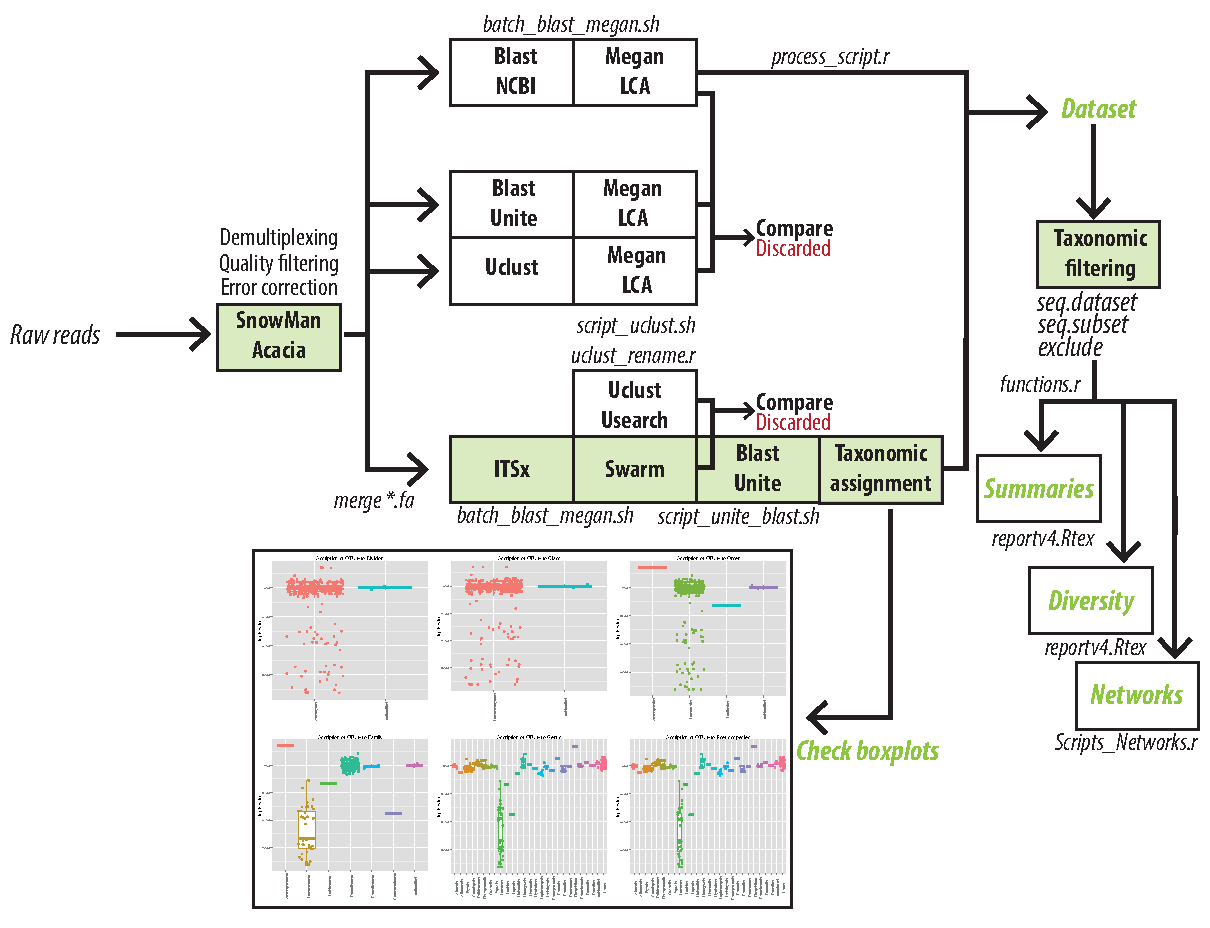
\includegraphics[width=\textwidth]{supplement_fig1.pdf}
  \caption{Schematic representation of the analytical pipeline. Files referred by filename can be found on the gitHub repository. Main pipeline is highlighted green and green names in italics highlight the main resulting data structures. Taxonomic filtering was done manually and included multiple manual and semiautomated validation steps.}
  \label{fig:supplement_fig1}
\end{figure}
\newpage
\section{Quality assesment and depth of the dataset used}
%--------------------------------%
%                                %
% INTRODUCTION                   %
%                                %
%--------------------------------%
\begin{knitrout}
\definecolor{shadecolor}{rgb}{0.969, 0.969, 0.969}\color{fgcolor}\begin{kframe}


{\ttfamily\noindent\itshape\color{messagecolor}{\#\# Loading required package: vegetarian}}\end{kframe}
\end{knitrout}
%
%------------------------------------------------------------------------------------------------%
%                                                                                                %
% 2nd CHUNK GETS AN OVERVIEW OF THE ITS1 DATASET AND PLOTS BOTH DATASETS IN ONE PLOT             %
%                                                                                                %
%------------------------------------------------------------------------------------------------%
% 
\begin{knitrout}
\definecolor{shadecolor}{rgb}{0.969, 0.969, 0.969}\color{fgcolor}\begin{figure}[H]
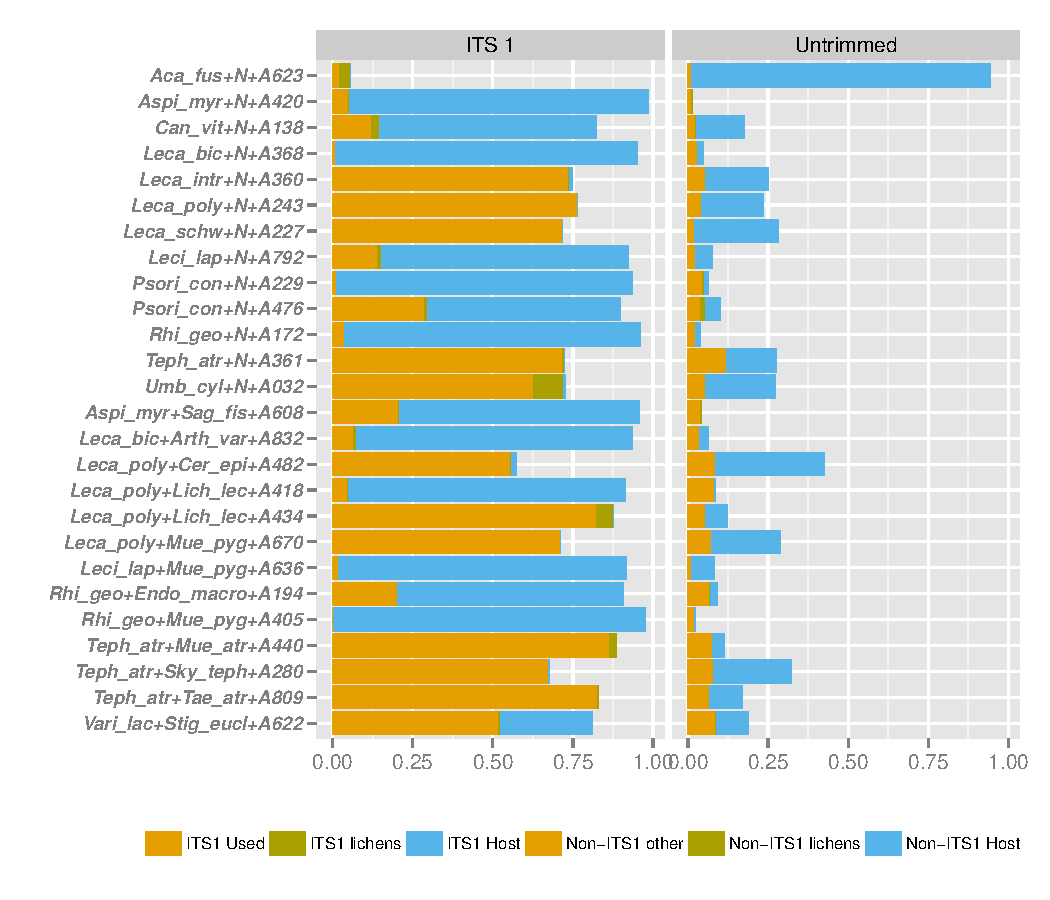
\includegraphics[width=\maxwidth]{figure/2_IntroAllNormalized-1} \caption[Overview of the trimmed (ITS1) and untrimmed datasets]{Overview of the trimmed (ITS1) and untrimmed datasets. The bars show the Proportion of reads per sample, and color codes the sequences that were included and excluded in each analysis}\label{fig:2_IntroAllNormalized}
\end{figure}


\end{knitrout}
%
%
%
% RAW READS
%
%
\begin{knitrout}
\definecolor{shadecolor}{rgb}{0.969, 0.969, 0.969}\color{fgcolor}\begin{figure}[H]
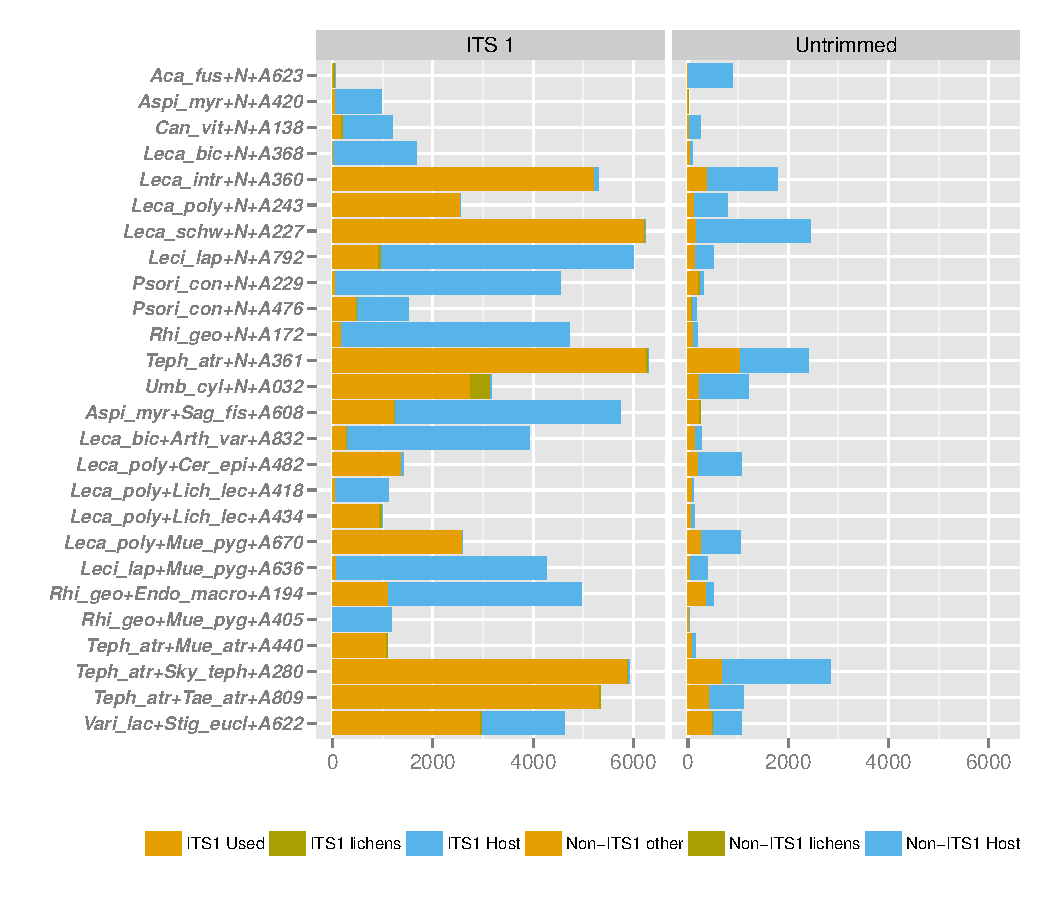
\includegraphics[width=\maxwidth]{figure/3_2_IntroReads-1} \caption[Overview of the trimmed (ITS1) and untrimmed datasets]{Overview of the trimmed (ITS1) and untrimmed datasets. The bars show the numer of reads per sample, and color codes the sequences that were included and excluded in each analysis}\label{fig:3_2_IntroReads}
\end{figure}


\end{knitrout}
%
% 4rd CHUNK GETS AN OVERVIEW OF THE ITS1 DATASET AND PLOTS BOTH DATASETS IN ONE PLOT
%
% TEXT ON QUALITY OF THE DATASET
%
%Analyses carried out in MEGAN including all quality filtered and dereplicated amplicons.\\
%Each sequence may include more an incomplete 5' fraction of SSU, including type I intronic sequences when present, ITS1 and 5.8S. When the type I intron is present the sequence of ITS1 is eaither partial or non existent.
%Unknown and Bacterial sequences are further interpreted as "unknown/unused".
%
%Representation of the dataset after being processes using ITSx. Sequences excluded because the do not contain ITS1 fractions are
%gruped as 11. 01 refers to sequences excluded for the analyses which contain ITS1 but are positively identified as belonging to one of the studied lichen hosts. 00 is the fraction of sequences included.\\
\newpage
\section{Taxonomic profile of the samples}
\subsection{Division}
%--------------------------------%
%                                %
% PLOT DIVISION COMPOSITION      %
%                                %
%--------------------------------%
\begin{knitrout}
\definecolor{shadecolor}{rgb}{0.969, 0.969, 0.969}\color{fgcolor}\begin{figure}[H]
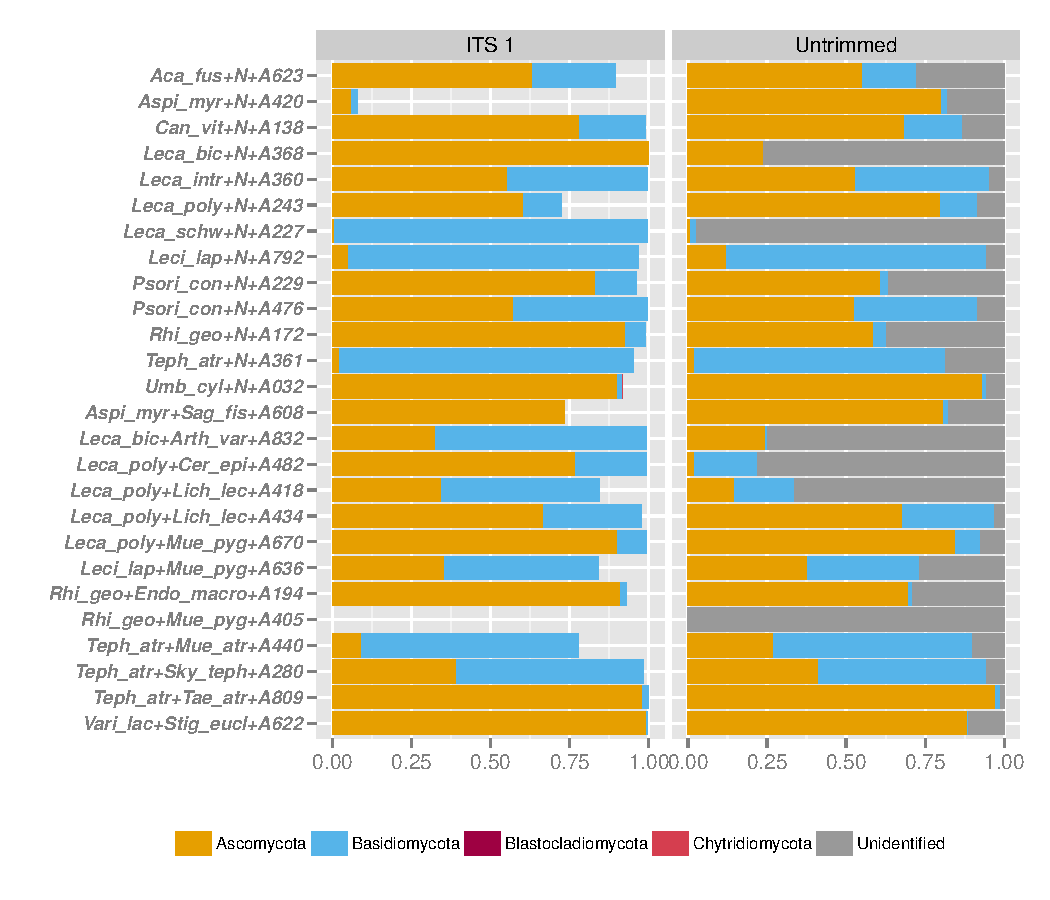
\includegraphics[width=\maxwidth]{figure/4_divisions-1} \caption[Overview of Taxonomic composition at Division level of the untrimmed dataset (SSU, Type I intron, ITS1, 5]{Overview of Taxonomic composition at Division level of the untrimmed dataset (SSU, Type I intron, ITS1, 5.8S) and the ITS1 dataset.}\label{fig:4_divisions}
\end{figure}


\end{knitrout}
%----------------------------------------------%
%                                              %
% PLOT TABLES OF DIVISION COMPOSITION          %
%                                              %
%----------------------------------------------%
% latex table generated in R 3.0.3 by xtable 1.7-4 package
% Mon Feb 20 14:09:36 2017
\begin{table}[H]
\centering
\caption[Divisions ITS1]{Number of raw reads asignable to Fungal Divisions in the ITS1 dataset} 
\begin{tabular}{rrrrr}
  \hline
 & Ascomycota & Basidiomycota & Chytridiomycota & unidentified \\ 
  \hline
Aca\_fus+N+A623 & 12 & 5 & . & 2 \\ 
  Aspi\_myr+N+A420 & 3 & 1 & . & 46 \\ 
  Can\_vit+N+A138 & 138 & 37 & . & 2 \\ 
  Leca\_bic+N+A368 & 16 & . & . & . \\ 
  Leca\_intr+N+A360 & 2885 & 2310 & . & 27 \\ 
  Leca\_poly+N+A243 & 1534 & 305 & . & 702 \\ 
  Leca\_schw+N+A227 & 42 & 6166 & . & 21 \\ 
  Leci\_lap+N+A792 & 47 & 836 & . & 31 \\ 
  Psori\_con+N+A229 & 44 & 7 & . & 2 \\ 
  Psori\_con+N+A476 & 275 & 205 & . & 2 \\ 
  Rhi\_geo+N+A172 & 162 & 11 & . & 2 \\ 
  Teph\_atr+N+A361 & 137 & 5823 & . & 306 \\ 
  Umb\_cyl+N+A032 & 2470 & 45 & 1 & 228 \\ 
  Aspi\_myr+Sag\_fis+A608 & 900 & . & . & 329 \\ 
  Leca\_bic+Arth\_var+A832 & 89 & 183 & . & 2 \\ 
  Leca\_poly+Cer\_epi+A482 & 1057 & 311 & . & 9 \\ 
  Leca\_poly+Lich\_lec+A418 & 20 & 29 & . & 9 \\ 
  Leca\_poly+Lich\_lec+A434 & 620 & 289 & . & 21 \\ 
  Leca\_poly+Mue\_pyg+A670 & 2330 & 237 & . & 22 \\ 
  Leci\_lap+Mue\_pyg+A636 & 29 & 40 & . & 13 \\ 
  Rhi\_geo+Endo\_macro+A194 & 1011 & 19 & . & 80 \\ 
  Rhi\_geo+Mue\_pyg+A405 & . & . & . & 2 \\ 
  Teph\_atr+Mue\_atr+A440 & 98 & 741 & . & 238 \\ 
  Teph\_atr+Sky\_teph+A280 & 2302 & 3486 & . & 100 \\ 
  Teph\_atr+Tae\_atr+A809 & 5229 & 88 & . & 13 \\ 
  Vari\_lac+Stig\_eucl+A622 & 2932 & 11 & . & 9 \\ 
   \hline
\end{tabular}
\end{table}


% latex table generated in R 3.0.3 by xtable 1.7-4 package
% Mon Feb 20 14:09:36 2017
\begin{table}[H]
\centering
\caption[Divisions MEGAN]{Number of reads asignable to Fungal Divisions in the untrimmed dataset} 
\begin{tabular}{rrrrr}
  \hline
 & Ascomycota & Basidiomycota & Blastocladiomycota & Unknown \\ 
  \hline
Aca\_fus+N+A623 & 16 & 5 & . & 8 \\ 
  Aspi\_myr+N+A420 & 49 & 1 & . & 11 \\ 
  Can\_vit+N+A138 & 146 & 39 & . & 28 \\ 
  Leca\_bic+N+A368 & 16 & . & . & 51 \\ 
  Leca\_intr+N+A360 & 2969 & 2374 & . & 263 \\ 
  Leca\_poly+N+A243 & 2139 & 314 & . & 223 \\ 
  Leca\_schw+N+A227 & 46 & 130 & . & 6228 \\ 
  Leci\_lap+N+A792 & 131 & 873 & . & 58 \\ 
  Psori\_con+N+A229 & 164 & 7 & . & 99 \\ 
  Psori\_con+N+A476 & 289 & 212 & . & 47 \\ 
  Rhi\_geo+N+A172 & 168 & 12 & . & 107 \\ 
  Teph\_atr+N+A361 & 142 & 5822 & . & 1358 \\ 
  Umb\_cyl+N+A032 & 2774 & 40 & 2 & 164 \\ 
  Aspi\_myr+Sag\_fis+A608 & 1178 & 22 & . & 259 \\ 
  Leca\_bic+Arth\_var+A832 & 104 & 3 & . & 318 \\ 
  Leca\_poly+Cer\_epi+A482 & 31 & 321 & . & 1239 \\ 
  Leca\_poly+Lich\_lec+A418 & 23 & 30 & . & 104 \\ 
  Leca\_poly+Lich\_lec+A434 & 673 & 291 & . & 29 \\ 
  Leca\_poly+Mue\_pyg+A670 & 2417 & 224 & . & 214 \\ 
  Leci\_lap+Mue\_pyg+A636 & 48 & 45 & . & 34 \\ 
  Rhi\_geo+Endo\_macro+A194 & 1036 & 19 & . & 430 \\ 
  Rhi\_geo+Mue\_pyg+A405 & . & . & . & 26 \\ 
  Teph\_atr+Mue\_atr+A440 & 317 & 741 & . & 116 \\ 
  Teph\_atr+Sky\_teph+A280 & 2708 & 3491 & . & 372 \\ 
  Teph\_atr+Tae\_atr+A809 & 5611 & 89 & . & 62 \\ 
  Vari\_lac+Stig\_eucl+A622 & 3047 & 11 & . & 389 \\ 
   \hline
\end{tabular}
\end{table}

\newpage
\subsection{Classes}
%
% PLOT IMAGES AND TABLES OF CLASS COMPOSITION
%
\begin{knitrout}
\definecolor{shadecolor}{rgb}{0.969, 0.969, 0.969}\color{fgcolor}\begin{figure}[H]
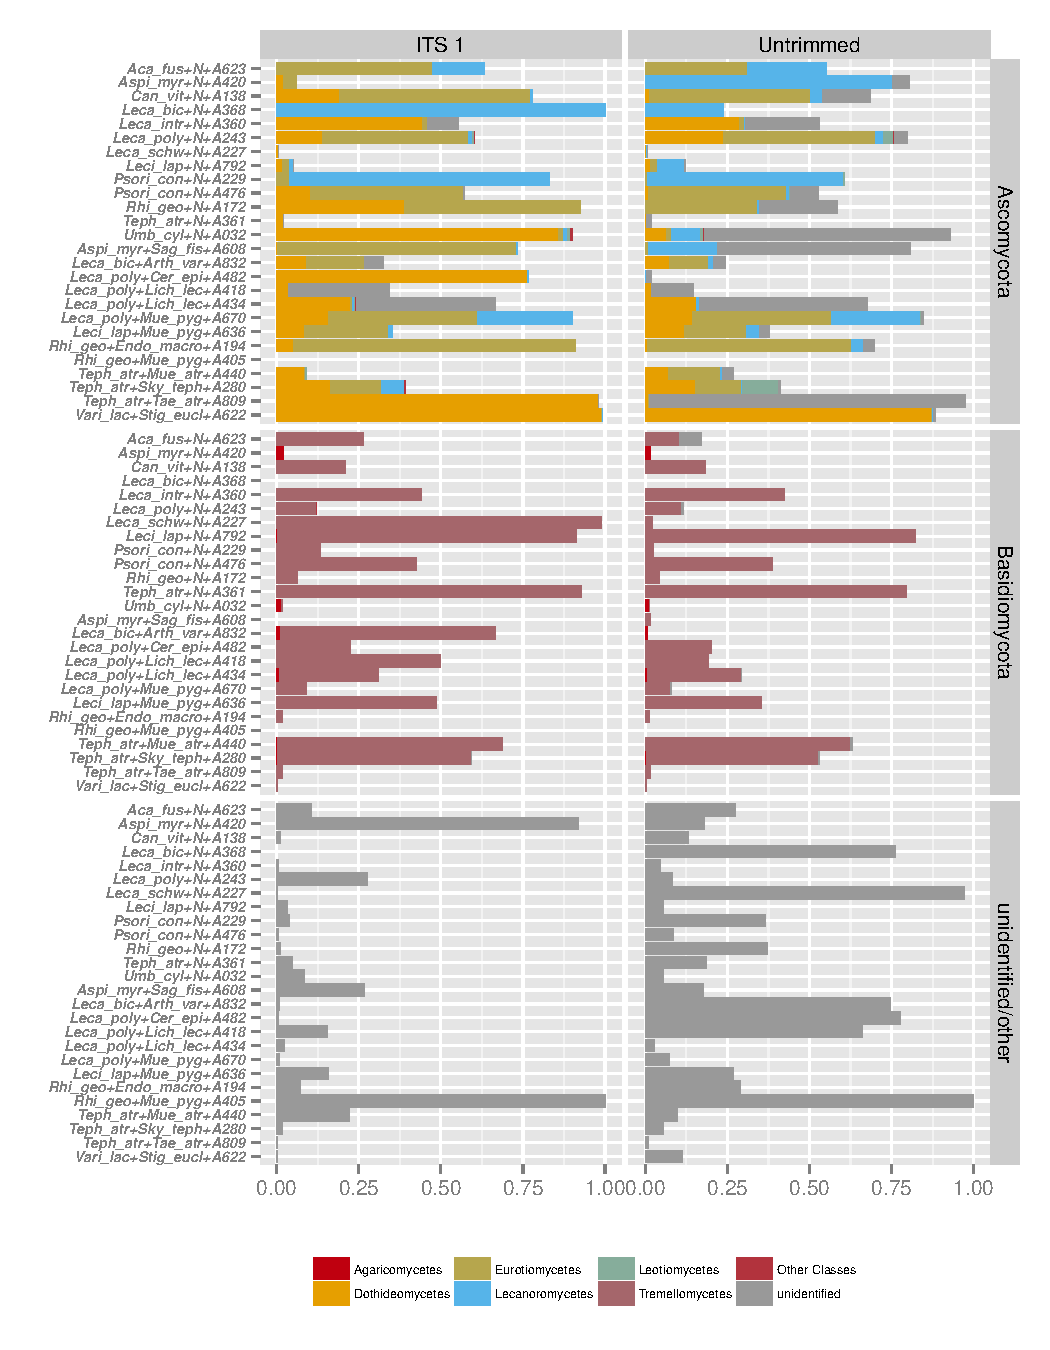
\includegraphics[width=\maxwidth]{figure/7_Class-1} \caption[Taxonomic composition at Class level of the untrimmed (SSU, Type I intron, ITS1, 5]{Taxonomic composition at Class level of the untrimmed (SSU, Type I intron, ITS1, 5.8S) and ITS1 datasets. Normalized fractions per sample are split by dataset and Division. The minoritary Blastocladiomycota and Chytridiomycota are grouped in the "unidentified/others" category }\label{fig:7_Class}
\end{figure}


\end{knitrout}
%
% CLASS TABLES
%
% latex table generated in R 3.0.3 by xtable 1.7-4 package
% Mon Feb 20 14:09:38 2017
\begin{sidewaystable}[b]
\centering
\caption[Classes ITS1]{Proportion of sequences asignable to Fungal Classes in the trimmed ITS1 dataset} 
\begin{tabular}{rrrrrrrrrrrrr}
  \hline
 & \begin{sideways} Dothideomycetes \end{sideways} & \begin{sideways} Eurotiomycetes \end{sideways} & \begin{sideways} Lecanoromycetes \end{sideways} & \begin{sideways} Leotiomycetes \end{sideways} & \begin{sideways} Saccharomycetes \end{sideways} & \begin{sideways} Sordariomycetes \end{sideways} & \begin{sideways} Taphrinomycetes \end{sideways} & \begin{sideways} Agaricomycetes \end{sideways} & \begin{sideways} Microbotryomycetes \end{sideways} & \begin{sideways} Tremellomycetes \end{sideways} & \begin{sideways} Blastocladiomycetes \end{sideways} & \begin{sideways} unidentified \end{sideways} \\ 
  \hline
Aca\_fus+N+A623 & . & 9 & 3 & . & . & . & . & . & . & 5 & . & 2 \\ 
  Aspi\_myr+N+A420 & 1 & 2 & . & . & . & . & . & 1 & . & . & . & 46 \\ 
  Can\_vit+N+A138 & 34 & 103 & 1 & . & . & . & . & . & . & 37 & . & 2 \\ 
  Leca\_bic+N+A368 & . & . & 16 & . & . & . & . & . & . & . & . & . \\ 
  Leca\_intr+N+A360 & 2326 & 77 & 1 & . & . & . & . & 1 & . & 2309 & . & 508 \\ 
  Leca\_poly+N+A243 & 358 & 1126 & 32 & 16 & . & 2 & . & 1 & 1 & 303 & . & 702 \\ 
  Leca\_schw+N+A227 & 26 & 10 & 3 & 1 & . & . & . & . & . & 6166 & . & 23 \\ 
  Leci\_lap+N+A792 & 16 & 20 & 10 & . & . & . & . & 1 & . & 835 & . & 32 \\ 
  Psori\_con+N+A229 & . & 2 & 42 & . & . & . & . & . & . & 7 & . & 2 \\ 
  Psori\_con+N+A476 & 50 & 224 & . & . & . & . & . & . & . & 205 & . & 3 \\ 
  Rhi\_geo+N+A172 & 68 & 94 & . & . & . & . & . & . & . & 11 & . & 2 \\ 
  Teph\_atr+N+A361 & 135 & 1 & . & . & . & . & . & . & . & 5823 & . & 307 \\ 
  Umb\_cyl+N+A032 & 2352 & 49 & 29 & 22 & 1 & 17 & . & 38 & . & 7 & 1 & 228 \\ 
  Aspi\_myr+Sag\_fis+A608 & 2 & 896 & 2 & . & . & . & . & . & . & . & . & 329 \\ 
  Leca\_bic+Arth\_var+A832 & 25 & 48 & . & . & . & . & . & 3 & . & 180 & . & 18 \\ 
  Leca\_poly+Cer\_epi+A482 & 1051 & 1 & 5 & . & . & . & . & . & . & 311 & . & 9 \\ 
  Leca\_poly+Lich\_lec+A418 & 2 & . & . & . & . & . & . & . & . & 29 & . & 27 \\ 
  Leca\_poly+Lich\_lec+A434 & 210 & 4 & 7 & 2 & . & 3 & . & 7 & . & 282 & . & 415 \\ 
  Leca\_poly+Mue\_pyg+A670 & 405 & 1177 & 748 & . & . & . & . & . & . & 237 & . & 22 \\ 
  Leci\_lap+Mue\_pyg+A636 & 7 & 21 & 1 & . & . & . & . & . & . & 40 & . & 13 \\ 
  Rhi\_geo+Endo\_macro+A194 & 56 & 955 & . & . & . & . & . & . & . & 19 & . & 80 \\ 
  Rhi\_geo+Mue\_pyg+A405 & . & . & . & . & . & . & . & . & . & . & . & 2 \\ 
  Teph\_atr+Mue\_atr+A440 & 90 & 4 & 1 & 3 & . & . & . & 1 & . & 740 & . & 238 \\ 
  Teph\_atr+Sky\_teph+A280 & 972 & 901 & 425 & . & . & . & 4 & 15 & . & 3470 & . & 101 \\ 
  Teph\_atr+Tae\_atr+A809 & 5226 & 2 & . & . & . & . & . & 1 & . & 87 & . & 14 \\ 
  Vari\_lac+Stig\_eucl+A622 & 2921 & 6 & 5 & . & . & . & . & 1 & . & 10 & . & 9 \\ 
   \hline
\end{tabular}
\end{sidewaystable}


% latex table generated in R 3.0.3 by xtable 1.7-4 package
% Mon Feb 20 14:09:38 2017
\begin{sidewaystable}[b]
\centering
\caption[Classes MEGAN]{Proportion of sequences asignable to Fungal Classes in the Complete dataset} 
\begin{tabular}{rrrrrrrrrrrrrrr}
  \hline
 & \begin{sideways} Dothideomycetes \end{sideways} & \begin{sideways} Eurotiomycetes \end{sideways} & \begin{sideways} Lecanoromycetes \end{sideways} & \begin{sideways} Leotiomycetes \end{sideways} & \begin{sideways} Orbiliomycetes \end{sideways} & \begin{sideways} Saccharomycetes \end{sideways} & \begin{sideways} Sordariomycetes \end{sideways} & \begin{sideways} Taphrinomycetes \end{sideways} & \begin{sideways} Agaricomycetes \end{sideways} & \begin{sideways} Agaricostilbomycetes \end{sideways} & \begin{sideways} Malasseziomycetes \end{sideways} & \begin{sideways} Tremellomycetes \end{sideways} & \begin{sideways} Blastocladiomycetes \end{sideways} & \begin{sideways} Unknown \end{sideways} \\ 
  \hline
Aca\_fus+N+A623 & . & 9 & 7 & . & . & . & . & . & . & . & . & 3 & . & 10 \\ 
  Aspi\_myr+N+A420 & . & . & 46 & . & . & . & . & . & 1 & . & . & . & . & 14 \\ 
  Can\_vit+N+A138 & 3 & 104 & 8 & . & . & . & . & . & . & . & . & 39 & . & 59 \\ 
  Leca\_bic+N+A368 & . & . & 16 & . & . & . & . & . & . & . & . & . & . & 51 \\ 
  Leca\_intr+N+A360 & 1613 & 80 & 10 & . & . & . & . & . & 1 & . & . & 2373 & . & 1529 \\ 
  Leca\_poly+N+A243 & 633 & 1242 & 69 & 76 & 9 & . & 2 & . & 1 & 1 & . & 292 & . & 351 \\ 
  Leca\_schw+N+A227 & 23 & 5 & 6 & 4 & . & . & . & . & . & . & . & 130 & . & 6236 \\ 
  Leci\_lap+N+A792 & 17 & 22 & 87 & . & . & . & . & . & 1 & . & . & 872 & . & 63 \\ 
  Psori\_con+N+A229 & . & 2 & 161 & 1 & . & . & . & . & . & . & . & 7 & . & 99 \\ 
  Psori\_con+N+A476 & 5 & 231 & 4 & 2 & . & . & . & . & . & . & . & 212 & . & 94 \\ 
  Rhi\_geo+N+A172 & . & 98 & 2 & . & . & . & . & . & . & . & . & 12 & . & 175 \\ 
  Teph\_atr+N+A361 & 19 & 1 & . & . & . & . & . & . & . & . & . & 5822 & . & 1480 \\ 
  Umb\_cyl+N+A032 & 190 & 43 & 269 & 22 & . & 2 & 7 & . & 39 & . & . & 1 & 2 & 2405 \\ 
  Aspi\_myr+Sag\_fis+A608 & 1 & 11 & 310 & . & . & . & . & . & . & . & . & 22 & . & 1115 \\ 
  Leca\_bic+Arth\_var+A832 & 31 & 51 & 6 & . & . & . & . & . & 3 & . & . & . & . & 334 \\ 
  Leca\_poly+Cer\_epi+A482 & 1 & 1 & 5 & . & . & . & . & . & . & . & . & 321 & . & 1263 \\ 
  Leca\_poly+Lich\_lec+A418 & 3 & . & . & . & . & . & . & . & . & . & . & 30 & . & 124 \\ 
  Leca\_poly+Lich\_lec+A434 & 154 & . & 10 & 1 & . & . & . & . & 7 & . & . & 283 & . & 538 \\ 
  Leca\_poly+Mue\_pyg+A670 & 408 & 1213 & 773 & 6 & . & . & 1 & . & . & . & . & 222 & . & 232 \\ 
  Leci\_lap+Mue\_pyg+A636 & 15 & 24 & 5 & . & . & . & . & . & . & . & . & 45 & . & 38 \\ 
  Rhi\_geo+Endo\_macro+A194 & 11 & 921 & 53 & . & . & . & . & . & . & . & . & 19 & . & 481 \\ 
  Rhi\_geo+Mue\_pyg+A405 & . & . & . & . & . & . & . & . & . & . & . & . & . & 26 \\ 
  Teph\_atr+Mue\_atr+A440 & 81 & 186 & 9 & 1 & . & . & . & . & . & . & . & 734 & . & 163 \\ 
  Teph\_atr+Sky\_teph+A280 & 1004 & 922 & 14 & 719 & . & . & . & 5 & 17 & . & 1 & 3452 & . & 437 \\ 
  Teph\_atr+Tae\_atr+A809 & 60 & 10 & 1 & . & . & . & . & . & 1 & . & . & 88 & . & 5602 \\ 
  Vari\_lac+Stig\_eucl+A622 & 3005 & 6 & 16 & 2 & . & . & . & . & 1 & . & . & 10 & . & 407 \\ 
   \hline
\end{tabular}
\end{sidewaystable}

%
%
%
\newpage
\subsection{Orders}
\begin{knitrout}
\definecolor{shadecolor}{rgb}{0.969, 0.969, 0.969}\color{fgcolor}\begin{figure}[H]
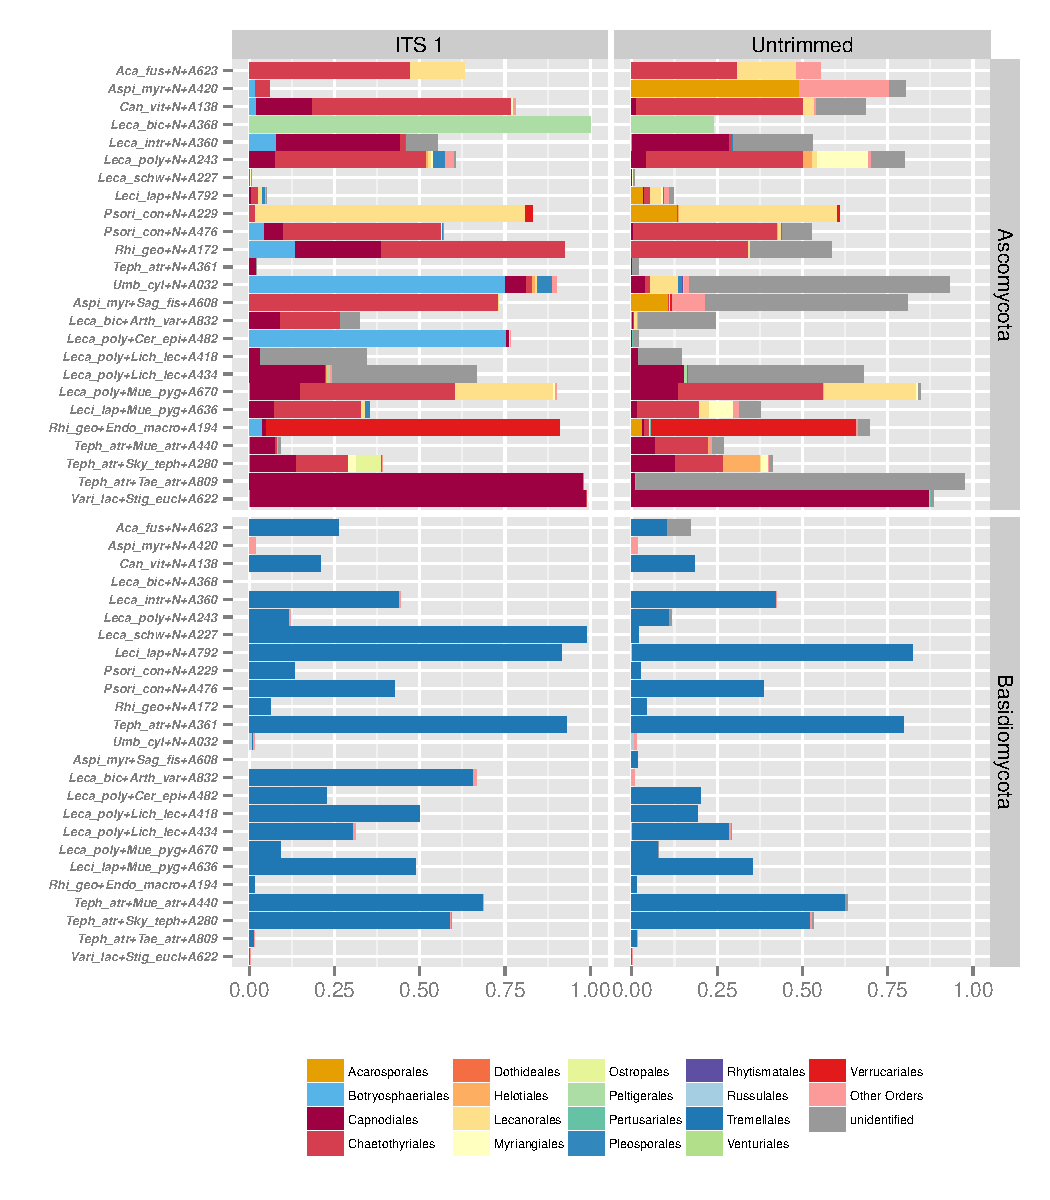
\includegraphics[width=\maxwidth]{figure/10_PlotOrders-1} \caption[Overview of Taxonomic composition at Order level split by dataset and Division]{Overview of Taxonomic composition at Order level split by dataset and Division.}\label{fig:10_PlotOrders}
\end{figure}


\end{knitrout}
%-------------------------------%
%                               %
% Tables Orders ITSX            %
%                               %
%-------------------------------%
% latex table generated in R 3.0.3 by xtable 1.7-4 package
% Mon Feb 20 14:09:40 2017
\begin{sidewaystable}[b]
\centering
\caption[Order ITS1 I]{Proportion of sequences asignable to Fungal Orders in the trimmed ITS1 dataset (Part I)} 
\begin{tabular}{rrrrrrrrrrrrrrrrrrr}
  \hline
 & \begin{sideways} Botryosphaeriales \end{sideways} & \begin{sideways} Candelariales \end{sideways} & \begin{sideways} Capnodiales \end{sideways} & \begin{sideways} Chaetothyriales \end{sideways} & \begin{sideways} Diaporthales \end{sideways} & \begin{sideways} Eurotiales \end{sideways} & \begin{sideways} Helotiales \end{sideways} & \begin{sideways} Hypocreales \end{sideways} & \begin{sideways} Lecanorales \end{sideways} & \begin{sideways} Lecideales \end{sideways} & \begin{sideways} Myriangiales \end{sideways} & \begin{sideways} Ostropales \end{sideways} & \begin{sideways} Peltigerales \end{sideways} & \begin{sideways} Pertusariales \end{sideways} & \begin{sideways} Pleosporales \end{sideways} & \begin{sideways} Rhizocarpales \end{sideways} & \begin{sideways} Saccharomycetales \end{sideways} & \begin{sideways} Taphrinales \end{sideways} \\ 
  \hline
Aca\_fus+N+A623 & . & . & . & 9 & . & . & . & . & 3 & . & . & . & . & . & . & . & . & . \\ 
  Aspi\_myr+N+A420 & 1 & . & . & 2 & . & . & . & . & . & . & . & . & . & . & . & . & . & . \\ 
  Can\_vit+N+A138 & 4 & . & 29 & 103 & . & . & . & . & . & . & 1 & . & . & . & . & 1 & . & . \\ 
  Leca\_bic+N+A368 & . & . & . & . & . & . & . & . & . & . & . & . & 16 & . & . & . & . & . \\ 
  Leca\_intr+N+A360 & 422 & . & 1900 & 76 & . & . & . & . & 1 & . & 1 & . & . & . & 3 & . & . & . \\ 
  Leca\_poly+N+A243 & 2 & 10 & 193 & 1126 & . & . & 16 & 59 & 19 & 1 & 17 & . & . & . & 89 & . & . & . \\ 
  Leca\_schw+N+A227 & 2 & . & 4 & 10 & . & . & 1 & . & 2 & . & 19 & 1 & . & . & 1 & . & . & . \\ 
  Leci\_lap+N+A792 & . & 1 & 6 & 20 & . & . & . & . & 9 & . & 1 & . & . & . & 9 & . & . & . \\ 
  Psori\_con+N+A229 & . & . & . & 1 & . & . & . & . & 42 & . & . & . & . & . & . & . & . & . \\ 
  Psori\_con+N+A476 & 21 & . & 27 & 224 & . & . & . & . & . & . & 1 & . & . & . & 1 & . & . & . \\ 
  Rhi\_geo+N+A172 & 24 & . & 44 & 94 & . & . & . & . & . & . & . & . & . & . & . & . & . & . \\ 
  Teph\_atr+N+A361 & 12 & . & 121 & 1 & . & . & . & . & . & . & . & . & . & . & 2 & . & . & . \\ 
  Umb\_cyl+N+A032 & 2063 & . & 169 & 49 & 6 & . & 22 & 11 & 14 & 7 & . & . & . & . & 120 & 7 & 1 & . \\ 
  Aspi\_myr+Sag\_fis+A608 & . & . & 2 & 896 & . & . & . & . & 2 & . & . & . & . & . & . & . & . & . \\ 
  Leca\_bic+Arth\_var+A832 & . & . & 25 & 48 & . & . & . & . & . & . & . & . & . & . & . & . & . & . \\ 
  Leca\_poly+Cer\_epi+A482 & 1038 & 1 & 13 & 1 & . & . & . & . & 3 & . & . & . & . & 1 & . & . & . & . \\ 
  Leca\_poly+Lich\_lec+A418 & . & . & 2 & . & . & . & . & . & . & . & . & . & . & . & . & . & . & . \\ 
  Leca\_poly+Lich\_lec+A434 & . & . & 208 & 4 & . & . & 2 & 3 & . & . & . & . & 7 & . & 2 & . & . & . \\ 
  Leca\_poly+Mue\_pyg+A670 & 9 & . & 379 & 1178 & . & . & . & . & 745 & . & 17 & . & . & . & . & 1 & . & . \\ 
  Leci\_lap+Mue\_pyg+A636 & . & . & 6 & 21 & . & . & . & . & 1 & . & . & . & . & . & 1 & . & . & . \\ 
  Rhi\_geo+Endo\_macro+A194 & 45 & . & 11 & 1 & . & . & . & . & . & . & . & . & . & . & . & . & . & . \\ 
  Rhi\_geo+Mue\_pyg+A405 & . & . & . & . & . & . & . & . & . & . & . & . & . & . & . & . & . & . \\ 
  Teph\_atr+Mue\_atr+A440 & 4 & . & 80 & 4 & . & . & 3 & . & . & . & . & . & . & . & . & . & . & . \\ 
  Teph\_atr+Sky\_teph+A280 & 30 & . & 785 & 899 & . & 2 & . & . & . & . & 146 & 424 & . & . & 11 & 1 & . & 4 \\ 
  Teph\_atr+Tae\_atr+A809 & . & . & 5225 & 2 & . & . & . & . & . & . & . & . & . & . & 1 & . & . & . \\ 
  Vari\_lac+Stig\_eucl+A622 & 14 & . & 2907 & 6 & . & . & . & . & 3 & . & . & 2 & . & . & . & . & . & . \\ 
   \hline
\end{tabular}
\end{sidewaystable}
% latex table generated in R 3.0.3 by xtable 1.7-4 package
% Mon Feb 20 14:09:40 2017
\begin{sidewaystable}[b]
\centering
\caption[Order ITS1 II]{Proportion of sequences asignable to Fungal Orders the trimmed ITS1 dataset (Part II)} 
\begin{tabular}{rrrrrrrrrrrrrrrr}
  \hline
 & \begin{sideways} Umbilicariales \end{sideways} & \begin{sideways} Verrucariales \end{sideways} & \begin{sideways} Agaricales \end{sideways} & \begin{sideways} Auriculariales \end{sideways} & \begin{sideways} Cantharellales \end{sideways} & \begin{sideways} Corticiales \end{sideways} & \begin{sideways} Cystofilobasidiales \end{sideways} & \begin{sideways} Hymenochaetales \end{sideways} & \begin{sideways} Polyporales \end{sideways} & \begin{sideways} Russulales \end{sideways} & \begin{sideways} Sebacinales \end{sideways} & \begin{sideways} Sporidiobolales \end{sideways} & \begin{sideways} Tremellales \end{sideways} & \begin{sideways} Blastocladiales \end{sideways} & \begin{sideways} unidentified \end{sideways} \\ 
  \hline
Aca\_fus+N+A623 & . & . & . & . & . & . & . & . & . & . & . & . & 5 & . & 2 \\ 
  Aspi\_myr+N+A420 & . & . & . & . & . & . & . & . & . & . & 1 & . & . & . & 46 \\ 
  Can\_vit+N+A138 & . & . & . & . & . & . & . & . & . & . & . & . & 37 & . & 2 \\ 
  Leca\_bic+N+A368 & . & . & . & . & . & . & . & . & . & . & . & . & . & . & . \\ 
  Leca\_intr+N+A360 & . & 1 & . & . & . & . & . & . & 1 & . & . & . & 2309 & . & 508 \\ 
  Leca\_poly+N+A243 & . & . & . & . & . & . & . & . & . & 1 & . & 1 & 303 & . & 704 \\ 
  Leca\_schw+N+A227 & . & . & . & . & . & . & . & . & . & . & . & . & 6166 & . & 23 \\ 
  Leci\_lap+N+A792 & . & . & . & . & . & . & . & . & . & 1 & . & . & 835 & . & 32 \\ 
  Psori\_con+N+A229 & . & 1 & . & . & . & . & . & . & . & . & . & . & 7 & . & 2 \\ 
  Psori\_con+N+A476 & . & . & . & . & . & . & . & . & . & . & . & . & 205 & . & 3 \\ 
  Rhi\_geo+N+A172 & . & . & . & . & . & . & . & . & . & . & . & . & 11 & . & 2 \\ 
  Teph\_atr+N+A361 & . & . & . & . & . & . & . & . & . & . & . & . & 5823 & . & 307 \\ 
  Umb\_cyl+N+A032 & 1 & . & 5 & . & 3 & . & . & . & 6 & 24 & . & . & 7 & 1 & 228 \\ 
  Aspi\_myr+Sag\_fis+A608 & . & . & . & . & . & . & . & . & . & . & . & . & . & . & 329 \\ 
  Leca\_bic+Arth\_var+A832 & . & . & 2 & . & . & . & . & 1 & . & . & . & . & 180 & . & 18 \\ 
  Leca\_poly+Cer\_epi+A482 & . & . & . & . & . & . & . & . & . & . & . & . & 311 & . & 9 \\ 
  Leca\_poly+Lich\_lec+A418 & . & . & . & . & . & . & . & . & . & . & . & . & 29 & . & 27 \\ 
  Leca\_poly+Lich\_lec+A434 & . & . & . & . & . & . & . & . & 5 & 2 & . & . & 282 & . & 415 \\ 
  Leca\_poly+Mue\_pyg+A670 & 1 & . & . & . & . & . & . & . & . & . & . & . & 237 & . & 22 \\ 
  Leci\_lap+Mue\_pyg+A636 & . & . & . & . & . & . & . & . & . & . & . & . & 40 & . & 13 \\ 
  Rhi\_geo+Endo\_macro+A194 & . & 954 & . & . & . & . & . & . & . & . & . & . & 19 & . & 80 \\ 
  Rhi\_geo+Mue\_pyg+A405 & . & . & . & . & . & . & . & . & . & . & . & . & . & . & 2 \\ 
  Teph\_atr+Mue\_atr+A440 & 1 & . & . & . & 1 & . & . & . & . & . & . & . & 740 & . & 244 \\ 
  Teph\_atr+Sky\_teph+A280 & . & . & 6 & 2 & . & 1 & 4 & 1 & 3 & 2 & . & . & 3466 & . & 101 \\ 
  Teph\_atr+Tae\_atr+A809 & . & . & . & . & . & . & . & 1 & . & . & . & . & 87 & . & 14 \\ 
  Vari\_lac+Stig\_eucl+A622 & . & . & 1 & . & . & . & . & . & . & . & . & . & 10 & . & 9 \\ 
   \hline
\end{tabular}
\end{sidewaystable}

\newpage
%
% Tables Orders MEGAN
%
% latex table generated in R 3.0.3 by xtable 1.7-4 package
% Mon Feb 20 14:09:40 2017
\begin{sidewaystable}[b]
\centering
\caption[Orders MEGAN I]{Proportion of sequences asignable to Fungal Orders in the untrimmed dataset (Part I)} 
\begin{tabular}{rrrrrrrrrrrrrrrrrrr}
  \hline
 & \begin{sideways} Acarosporales \end{sideways} & \begin{sideways} Candelariales \end{sideways} & \begin{sideways} Capnodiales \end{sideways} & \begin{sideways} Chaetothyriales \end{sideways} & \begin{sideways} Diaporthales \end{sideways} & \begin{sideways} Dothideales \end{sideways} & \begin{sideways} Eurotiales \end{sideways} & \begin{sideways} Helotiales \end{sideways} & \begin{sideways} Hypocreales \end{sideways} & \begin{sideways} Lecanorales \end{sideways} & \begin{sideways} Lecideales \end{sideways} & \begin{sideways} Myriangiales \end{sideways} & \begin{sideways} Orbiliales \end{sideways} & \begin{sideways} Peltigerales \end{sideways} & \begin{sideways} Pertusariales \end{sideways} & \begin{sideways} Phacidiales \end{sideways} & \begin{sideways} Phaeomoniellales \end{sideways} & \begin{sideways} Pleosporales \end{sideways} \\ 
  \hline
Aca\_fus+N+A623 & . & . & . & 9 & . & . & . & . & . & 5 & . & . & . & . & . & . & . & . \\ 
  Aspi\_myr+N+A420 & 30 & . & . & . & . & . & . & . & . & . & . & . & . & . & . & . & . & . \\ 
  Can\_vit+N+A138 & . & . & 3 & 104 & . & . & . & . & . & 7 & . & . & . & . & . & . & . & . \\ 
  Leca\_bic+N+A368 & . & . & . & . & . & . & . & . & . & . & . & . & . & 16 & . & . & . & . \\ 
  Leca\_intr+N+A360 & 2 & . & 1610 & 40 & . & . & . & . & . & 7 & . & 1 & . & . & . & . & 1 & 2 \\ 
  Leca\_poly+N+A243 & . & . & 116 & 1232 & . & . & . & 69 & 2 & 43 & 1 & 394 & 9 & . & . & . & 9 & . \\ 
  Leca\_schw+N+A227 & . & 1 & 4 & 5 & . & . & . & 4 & . & 5 & . & 18 & . & . & . & . & . & 1 \\ 
  Leci\_lap+N+A792 & 36 & 14 & 2 & 20 & . & . & . & . & . & 35 & . & 6 & . & . & . & . & 2 & 1 \\ 
  Psori\_con+N+A229 & 36 & . & . & 1 & . & . & . & 1 & . & 125 & . & . & . & . & . & . & . & . \\ 
  Psori\_con+N+A476 & . & . & 3 & 231 & . & . & . & 2 & . & 4 & . & 1 & . & . & . & . & . & 1 \\ 
  Rhi\_geo+N+A172 & . & . & . & 98 & . & . & . & . & . & 2 & . & . & . & . & . & . & . & . \\ 
  Teph\_atr+N+A361 & . & . & 17 & 1 & . & . & . & . & . & . & . & . & . & . & . & . & . & . \\ 
  Umb\_cyl+N+A032 & . & . & 119 & 40 & 6 & 1 & . & 1 & 1 & 246 & 7 & . & . & 1 & . & 9 & . & 35 \\ 
  Aspi\_myr+Sag\_fis+A608 & 158 & . & . & 3 & . & 1 & . & . & . & 2 & . & . & . & . & . & . & . & . \\ 
  Leca\_bic+Arth\_var+A832 & 1 & . & 1 & 1 & . & . & . & . & . & 4 & . & . & . & . & . & . & . & . \\ 
  Leca\_poly+Cer\_epi+A482 & . & . & 1 & 1 & . & . & . & . & . & 3 & . & . & . & . & 2 & . & . & . \\ 
  Leca\_poly+Lich\_lec+A418 & . & . & 3 & . & . & . & . & . & . & . & . & . & . & . & . & . & . & . \\ 
  Leca\_poly+Lich\_lec+A434 & . & . & 152 & . & . & . & . & 1 & . & 1 & . & . & . & 8 & . & . & . & 2 \\ 
  Leca\_poly+Mue\_pyg+A670 & . & . & 391 & 1213 & . & . & . & 6 & 1 & 769 & . & 17 & . & . & . & . & . & . \\ 
  Leci\_lap+Mue\_pyg+A636 & . & . & 2 & 23 & . & . & . & . & . & 4 & 1 & 9 & . & . & . & . & 1 & . \\ 
  Rhi\_geo+Endo\_macro+A194 & 45 & . & 11 & 21 & . & . & 5 & . & . & 5 & . & . & . & . & 2 & . & . & . \\ 
  Rhi\_geo+Mue\_pyg+A405 & . & . & . & . & . & . & . & . & . & . & . & . & . & . & . & . & . & . \\ 
  Teph\_atr+Mue\_atr+A440 & . & . & 81 & 184 & . & . & . & 1 & . & . & . & . & . & . & . & . & . & . \\ 
  Teph\_atr+Sky\_teph+A280 & 2 & 2 & 845 & 920 & . & . & 2 & 719 & . & 5 & . & 146 & . & . & . & . & . & 4 \\ 
  Teph\_atr+Tae\_atr+A809 & . & . & 59 & 10 & . & . & . & . & . & . & . & . & . & . & 1 & . & . & 1 \\ 
  Vari\_lac+Stig\_eucl+A622 & . & . & 3005 & 6 & . & . & . & 2 & . & 8 & . & . & . & . & 8 & . & . & . \\ 
   \hline
\end{tabular}
\end{sidewaystable}
% latex table generated in R 3.0.3 by xtable 1.7-4 package
% Mon Feb 20 14:09:40 2017
\begin{sidewaystable}[b]
\centering
\caption[Orders MEGAN II]{Proportion of sequences asignable to Fungal Orders in the untrimmed dataset  (Part II)} 
\begin{tabular}{rrrrrrrrrrrrrrrrrrrrrr}
  \hline
 & \begin{sideways} Rhizocarpales \end{sideways} & \begin{sideways} Rhytismatales \end{sideways} & \begin{sideways} Saccharomycetales \end{sideways} & \begin{sideways} Taphrinales \end{sideways} & \begin{sideways} Trapeliales \end{sideways} & \begin{sideways} Umbilicariales \end{sideways} & \begin{sideways} Venturiales \end{sideways} & \begin{sideways} Verrucariales \end{sideways} & \begin{sideways} Agaricales \end{sideways} & \begin{sideways} Auriculariales \end{sideways} & \begin{sideways} Corticiales \end{sideways} & \begin{sideways} Cystofilobasidiales \end{sideways} & \begin{sideways} Holtermanniales \end{sideways} & \begin{sideways} Hymenochaetales \end{sideways} & \begin{sideways} Malasseziales \end{sideways} & \begin{sideways} Polyporales \end{sideways} & \begin{sideways} Russulales \end{sideways} & \begin{sideways} Sebacinales \end{sideways} & \begin{sideways} Tremellales \end{sideways} & \begin{sideways} Blastocladiales \end{sideways} & \begin{sideways} Unknown \end{sideways} \\ 
  \hline
Aca\_fus+N+A623 & 2 & . & . & . & . & . & . & . & . & . & . & . & . & . & . & . & . & . & 3 & . & 10 \\ 
  Aspi\_myr+N+A420 & . & . & . & . & . & 16 & . & . & . & . & . & . & . & . & . & . & . & 1 & . & . & 14 \\ 
  Can\_vit+N+A138 & 1 & . & . & . & . & . & . & . & . & . & . & . & . & . & . & . & . & . & 39 & . & 59 \\ 
  Leca\_bic+N+A368 & . & . & . & . & . & . & . & . & . & . & . & . & . & . & . & . & . & . & . & . & 51 \\ 
  Leca\_intr+N+A360 & 1 & . & . & . & . & . & . & 1 & . & . & . & . & . & . & . & 1 & . & . & 2373 & . & 1567 \\ 
  Leca\_poly+N+A243 & . & . & . & . & . & . & 1 & 1 & . & . & . & . & . & 1 & . & . & . & . & 292 & . & 506 \\ 
  Leca\_schw+N+A227 & . & . & . & . & . & . & . & . & . & . & . & . & . & . & . & . & . & . & 130 & . & 6236 \\ 
  Leci\_lap+N+A792 & . & . & . & . & . & 2 & . & . & . & . & . & . & . & . & . & . & 1 & . & 872 & . & 71 \\ 
  Psori\_con+N+A229 & . & . & . & . & . & . & . & 1 & . & . & . & . & . & . & . & . & . & . & 7 & . & 99 \\ 
  Psori\_con+N+A476 & . & . & . & . & . & . & . & . & . & . & . & . & . & . & . & . & . & . & 212 & . & 94 \\ 
  Rhi\_geo+N+A172 & . & . & . & . & . & . & . & . & . & . & . & . & . & . & . & . & . & . & 12 & . & 175 \\ 
  Teph\_atr+N+A361 & . & . & . & . & . & . & . & . & . & . & . & . & . & . & . & . & . & . & 5822 & . & 1482 \\ 
  Umb\_cyl+N+A032 & 14 & 12 & 2 & . & . & 1 & 8 & . & 5 & . & 3 & . & 1 & . & . & 6 & 25 & . & . & 2 & 2435 \\ 
  Aspi\_myr+Sag\_fis+A608 & . & . & . & . & . & 143 & . & 8 & . & . & . & . & . & . & . & . & . & . & 22 & . & 1122 \\ 
  Leca\_bic+Arth\_var+A832 & . & . & . & . & . & 1 & . & . & 2 & . & . & . & . & 1 & . & . & . & . & . & . & 414 \\ 
  Leca\_poly+Cer\_epi+A482 & . & . & . & . & . & . & . & . & . & . & . & . & . & . & . & . & . & . & 321 & . & 1263 \\ 
  Leca\_poly+Lich\_lec+A418 & . & . & . & . & . & . & . & . & . & . & . & . & . & . & . & . & . & . & 30 & . & 124 \\ 
  Leca\_poly+Lich\_lec+A434 & . & . & . & . & . & 1 & . & . & . & . & . & . & . & . & . & 5 & 2 & . & 283 & . & 538 \\ 
  Leca\_poly+Mue\_pyg+A670 & 1 & . & . & . & . & 3 & . & . & . & . & . & . & . & . & . & . & . & . & 222 & . & 232 \\ 
  Leci\_lap+Mue\_pyg+A636 & . & . & . & . & . & . & . & . & . & . & . & . & . & . & . & . & . & . & 45 & . & 42 \\ 
  Rhi\_geo+Endo\_macro+A194 & . & . & . & . & . & 1 & . & 895 & . & . & . & . & . & . & . & . & . & . & 19 & . & 481 \\ 
  Rhi\_geo+Mue\_pyg+A405 & . & . & . & . & . & . & . & . & . & . & . & . & . & . & . & . & . & . & . & . & 26 \\ 
  Teph\_atr+Mue\_atr+A440 & 8 & . & . & . & . & 1 & . & 2 & . & . & . & . & . & . & . & . & . & . & 734 & . & 163 \\ 
  Teph\_atr+Sky\_teph+A280 & 1 & . & . & 5 & 2 & 2 & . & . & 7 & 2 & 2 & 4 & . & . & 1 & 4 & 2 & . & 3448 & . & 446 \\ 
  Teph\_atr+Tae\_atr+A809 & . & . & . & . & . & . & . & . & . & . & . & . & . & 1 & . & . & . & . & 88 & . & 5602 \\ 
  Vari\_lac+Stig\_eucl+A622 & . & . & . & . & . & . & . & . & 1 & . & . & . & . & . & . & . & . & . & 10 & . & 407 \\ 
   \hline
\end{tabular}
\end{sidewaystable}

\subsection{Families}
%
% PLOT OF FAMILY ASCRIPTION
%
\begin{knitrout}
\definecolor{shadecolor}{rgb}{0.969, 0.969, 0.969}\color{fgcolor}\begin{figure}[H]
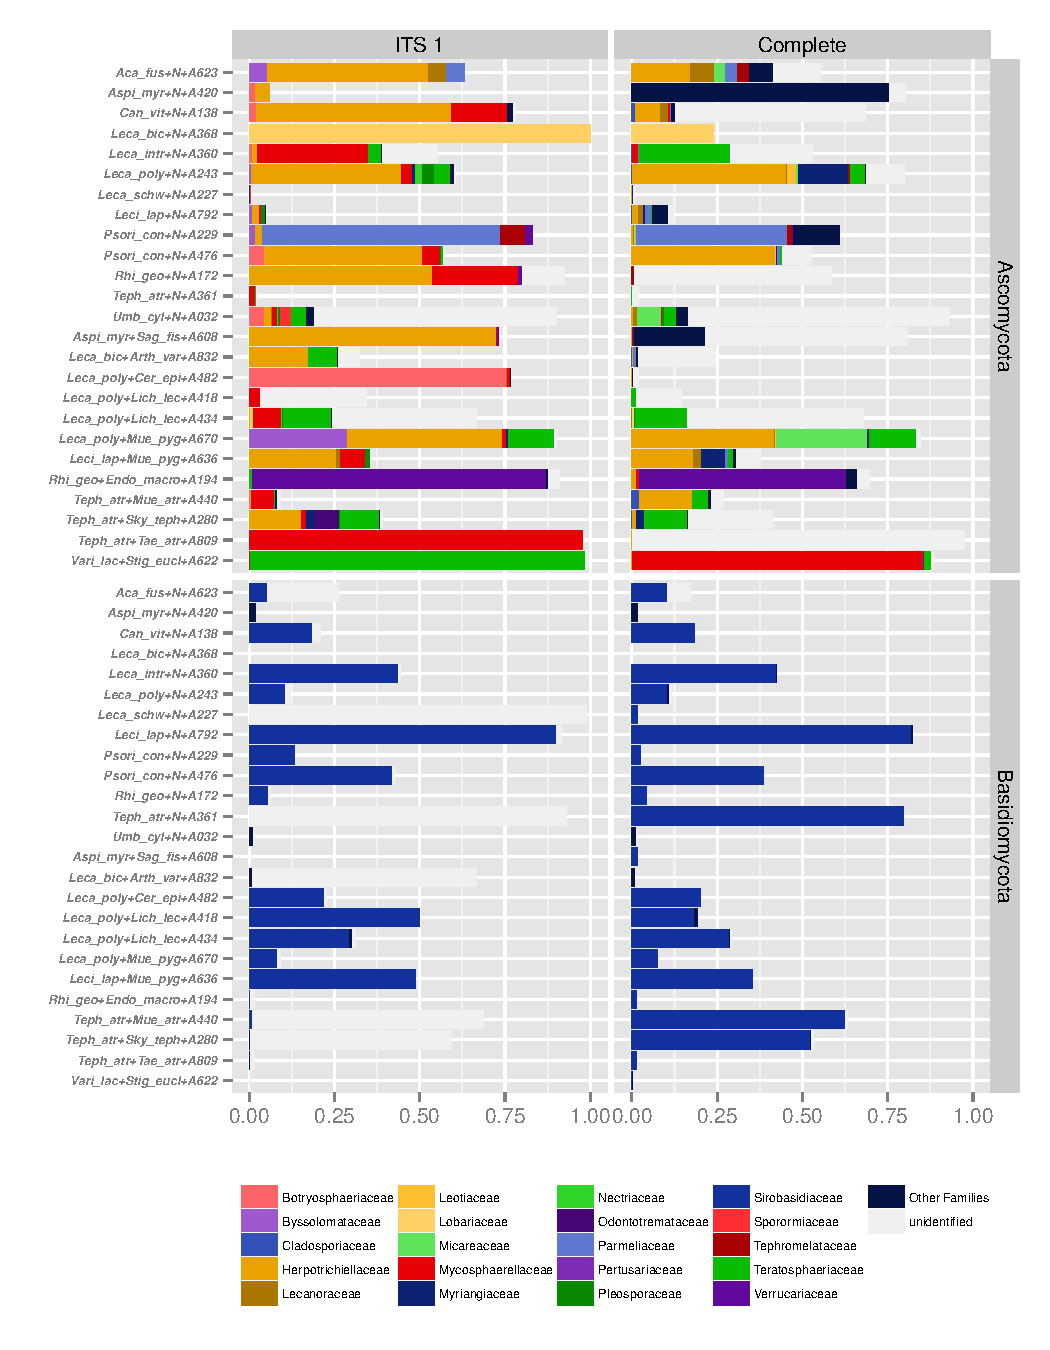
\includegraphics[width=\maxwidth]{figure/14_PlotFamilies-1} \caption[Overview of Taxonomic composition at Family level split by dataset and Division]{Overview of Taxonomic composition at Family level split by dataset and Division. Minoritary Families within Asco and Basidiomycota were recoded as "other" for graphical simplicity. Full Results can be found in tables X:Y}\label{fig:14_PlotFamilies}
\end{figure}


\end{knitrout}
%<<14_PlotFamilieslegend, echo=FALSE, fig.height=4, fig.width=4, fig.pos='H'>>=
%plot(g_legend(mof))
%@
\newpage
%
% TABLE FAMILIES ITS1
%
% latex table generated in R 3.0.3 by xtable 1.7-4 package
% Mon Feb 20 14:09:42 2017
\begin{sidewaystable}[b]
\centering
\caption[Families ITS1 I]{Proportion of sequences asignable to Fungal Families the trimmed ITS1 dataset (Part I)} 
\begin{tabular}{rrrrrrrrrrrrrrrrrrr}
  \hline
 & \begin{sideways} Botryosphaeriaceae \end{sideways} & \begin{sideways} Byssolomataceae \end{sideways} & \begin{sideways} Candelariaceae \end{sideways} & \begin{sideways} Catenariaceae \end{sideways} & \begin{sideways} Chaetothyriaceae \end{sideways} & \begin{sideways} Chionosphaeraceae \end{sideways} & \begin{sideways} Corticiaceae \end{sideways} & \begin{sideways} Cystofilobasidiaceae \end{sideways} & \begin{sideways} Davidiellaceae \end{sideways} & \begin{sideways} Dermateaceae \end{sideways} & \begin{sideways} Filobasidiaceae \end{sideways} & \begin{sideways} Fomitopsidaceae \end{sideways} & \begin{sideways} Ganodermataceae \end{sideways} & \begin{sideways} Helotiaceae \end{sideways} & \begin{sideways} Hemiphacidiaceae \end{sideways} & \begin{sideways} Herpotrichiellaceae \end{sideways} & \begin{sideways} Hyaloscyphaceae \end{sideways} & \begin{sideways} Hydnaceae \end{sideways} \\ 
  \hline
Aca\_fus+N+A623 & . & 1 & . & . & . & . & . & . & . & . & . & . & . & . & . & 9 & . & . \\ 
  Aspi\_myr+N+A420 & 1 & . & . & . & . & . & . & . & . & . & . & . & . & . & . & 2 & . & . \\ 
  Can\_vit+N+A138 & 4 & . & . & . & 2 & . & . & . & . & . & . & . & . & . & . & 101 & . & . \\ 
  Leca\_bic+N+A368 & . & . & . & . & . & . & . & . & . & . & . & . & . & . & . & . & . & . \\ 
  Leca\_intr+N+A360 & 53 & . & . & . & . & . & . & . & 4 & . & . & . & . & . & . & 77 & . & . \\ 
  Leca\_poly+N+A243 & . & 14 & 10 & . & . & 1 & . & . & 1 & 8 & 2 & . & . & . & . & 1123 & 7 & . \\ 
  Leca\_schw+N+A227 & 1 & . & . & . & . & . & . & . & 2 & . & . & . & . & . & . & 10 & . & . \\ 
  Leci\_lap+N+A792 & . & 8 & 1 & . & . & . & . & . & 1 & . & . & . & . & . & . & 20 & . & . \\ 
  Psori\_con+N+A229 & . & 1 & . & . & . & . & . & . & . & . & . & . & . & . & . & 1 & . & . \\ 
  Psori\_con+N+A476 & 21 & . & . & . & . & . & . & . & . & . & . & . & . & . & . & 224 & . & . \\ 
  Rhi\_geo+N+A172 & . & . & . & . & . & . & . & . & . & . & . & . & . & . & . & 94 & . & . \\ 
  Teph\_atr+N+A361 & 9 & . & . & . & . & . & . & . & 1 & . & . & . & . & . & . & 1 & . & . \\ 
  Umb\_cyl+N+A032 & 127 & . & . & 1 & . & . & . & . & . & . & . & 1 & 3 & 1 & 12 & 49 & . & 3 \\ 
  Aspi\_myr+Sag\_fis+A608 & . & . & . & . & . & . & . & . & . & . & . & . & . & . & . & 891 & . & . \\ 
  Leca\_bic+Arth\_var+A832 & . & . & . & . & . & . & . & . & 1 & . & . & . & . & . & . & 48 & . & . \\ 
  Leca\_poly+Cer\_epi+A482 & 1038 & 1 & 1 & . & . & . & . & . & . & . & . & . & . & . & . & 1 & . & . \\ 
  Leca\_poly+Lich\_lec+A418 & . & . & . & . & . & . & . & . & . & . & . & . & . & . & . & . & . & . \\ 
  Leca\_poly+Lich\_lec+A434 & . & . & . & . & . & . & . & . & . & . & . & . & . & . & 1 & 4 & . & . \\ 
  Leca\_poly+Mue\_pyg+A670 & . & 744 & . & . & . & . & . & . & . & . & . & . & . & . & . & 1178 & . & . \\ 
  Leci\_lap+Mue\_pyg+A636 & . & . & . & . & . & . & . & . & . & . & . & . & . & . & . & 21 & . & . \\ 
  Rhi\_geo+Endo\_macro+A194 & . & . & . & . & . & . & . & . & . & . & . & . & . & . & . & 1 & . & . \\ 
  Rhi\_geo+Mue\_pyg+A405 & . & . & . & . & . & . & . & . & . & . & . & . & . & . & . & . & . & . \\ 
  Teph\_atr+Mue\_atr+A440 & 4 & . & . & . & . & . & . & . & 1 & . & . & . & . & . & . & 4 & 3 & . \\ 
  Teph\_atr+Sky\_teph+A280 & 1 & . & . & . & . & . & 1 & 4 & 5 & . & . & . & . & . & . & 897 & . & . \\ 
  Teph\_atr+Tae\_atr+A809 & . & . & . & . & . & . & . & . & . & . & . & . & . & . & . & 2 & . & . \\ 
  Vari\_lac+Stig\_eucl+A622 & . & . & . & . & . & . & . & . & 1 & . & . & . & . & . & . & 3 & . & . \\ 
   \hline
\end{tabular}
\end{sidewaystable}
% latex table generated in R 3.0.3 by xtable 1.7-4 package
% Mon Feb 20 14:09:42 2017
\begin{sidewaystable}[b]
\centering
\caption[Families ITS1 II]{Proportion of sequences asignable to Fungal Families the trimmed ITS1 dataset (Part II)} 
\begin{tabular}{rrrrrrrrrrrrrrrrrrrr}
  \hline
 & \begin{sideways} Hymenochaetaceae \end{sideways} & \begin{sideways} Lecanoraceae \end{sideways} & \begin{sideways} Lecideaceae \end{sideways} & \begin{sideways} Leptosphaeriaceae \end{sideways} & \begin{sideways} Lobariaceae \end{sideways} & \begin{sideways} Marasmiaceae \end{sideways} & \begin{sideways} Megasporaceae \end{sideways} & \begin{sideways} Melanommataceae \end{sideways} & \begin{sideways} Meruliaceae \end{sideways} & \begin{sideways} Mycenaceae \end{sideways} & \begin{sideways} Mycosphaerellaceae \end{sideways} & \begin{sideways} Myriangiaceae \end{sideways} & \begin{sideways} Nectriaceae \end{sideways} & \begin{sideways} Odontotremataceae \end{sideways} & \begin{sideways} Ophiocordycipitaceae \end{sideways} & \begin{sideways} Ophioparmaceae \end{sideways} & \begin{sideways} Parmeliaceae \end{sideways} & \begin{sideways} Peniophoraceae \end{sideways} & \begin{sideways} Phacidiaceae \end{sideways} \\ 
  \hline
Aca\_fus+N+A623 & . & 1 & . & . & . & . & . & . & . & . & . & . & . & . & . & . & 1 & . & . \\ 
  Aspi\_myr+N+A420 & . & . & . & . & . & . & . & . & . & . & . & . & . & . & . & . & . & . & . \\ 
  Can\_vit+N+A138 & . & . & . & . & . & . & . & . & . & . & 29 & . & . & . & . & . & . & . & . \\ 
  Leca\_bic+N+A368 & . & . & . & . & 16 & . & . & . & . & . & . & . & . & . & . & . & . & . & . \\ 
  Leca\_intr+N+A360 & . & . & . & 1 & . & . & . & . & . & . & 1694 & 1 & . & . & . & . & 1 & . & . \\ 
  Leca\_poly+N+A243 & . & 1 & 1 & . & . & . & . & 1 & . & . & 81 & 17 & 57 & . & 2 & . & 1 & 1 & . \\ 
  Leca\_schw+N+A227 & . & 1 & . & . & . & . & . & . & . & . & 1 & 19 & . & 1 & . & . & . & . & . \\ 
  Leci\_lap+N+A792 & . & . & . & . & . & . & . & . & . & . & 4 & 1 & . & . & . & . & 1 & 1 & . \\ 
  Psori\_con+N+A229 & . & . & . & . & . & . & . & . & . & . & . & . & . & . & . & . & 37 & . & . \\ 
  Psori\_con+N+A476 & . & . & . & . & . & . & . & . & . & . & 25 & 1 & . & . & . & . & . & . & . \\ 
  Rhi\_geo+N+A172 & . & . & . & . & . & . & . & . & . & . & 44 & . & . & . & . & . & . & . & . \\ 
  Teph\_atr+N+A361 & . & . & . & . & . & . & . & . & . & . & 112 & . & . & . & . & . & . & . & . \\ 
  Umb\_cyl+N+A032 & . & 13 & 7 & . & . & . & . & 16 & . & . & 38 & . & 11 & . & . & 1 & 1 & . & 9 \\ 
  Aspi\_myr+Sag\_fis+A608 & . & . & . & . & . & . & . & . & . & . & 2 & . & . & . & . & . & . & . & . \\ 
  Leca\_bic+Arth\_var+A832 & 1 & . & . & . & . & 2 & . & . & . & . & . & . & . & . & . & . & . & . & . \\ 
  Leca\_poly+Cer\_epi+A482 & . & 2 & . & . & . & . & 1 & . & . & . & 13 & . & . & . & . & . & . & . & . \\ 
  Leca\_poly+Lich\_lec+A418 & . & . & . & . & . & . & . & . & . & . & 2 & . & . & . & . & . & . & . & . \\ 
  Leca\_poly+Lich\_lec+A434 & . & . & . & . & 7 & . & . & . & 2 & . & 77 & . & 3 & . & . & . & . & 2 & . \\ 
  Leca\_poly+Mue\_pyg+A670 & . & . & . & . & . & . & . & . & . & . & 32 & 17 & . & . & . & . & . & . & . \\ 
  Leci\_lap+Mue\_pyg+A636 & . & 1 & . & . & . & . & . & . & . & . & 6 & . & . & . & . & . & . & . & . \\ 
  Rhi\_geo+Endo\_macro+A194 & . & . & . & . & . & . & 8 & . & . & . & . & . & . & . & . & . & . & . & . \\ 
  Rhi\_geo+Mue\_pyg+A405 & . & . & . & . & . & . & . & . & . & . & . & . & . & . & . & . & . & . & . \\ 
  Teph\_atr+Mue\_atr+A440 & . & . & . & . & . & . & . & . & . & . & 71 & . & . & . & . & . & . & . & . \\ 
  Teph\_atr+Sky\_teph+A280 & . & . & . & . & . & 1 & . & . & 2 & 1 & 96 & 146 & . & 424 & . & . & . & 2 & . \\ 
  Teph\_atr+Tae\_atr+A809 & . & . & . & . & . & . & . & . & . & . & 5222 & . & . & . & . & . & . & . & . \\ 
  Vari\_lac+Stig\_eucl+A622 & . & 2 & . & . & . & . & . & . & . & . & 6 & . & . & 2 & . & . & 1 & . & . \\ 
   \hline
\end{tabular}
\end{sidewaystable}
% latex table generated in R 3.0.3 by xtable 1.7-4 package
% Mon Feb 20 14:09:42 2017
\begin{sidewaystable}[b]
\centering
\caption[Families ITS1 III]{Proportion of sequences asignable to Fungal Families the trimmed ITS1 dataset (Part III)} 
\begin{tabular}{rrrrrrrrrrrrrrrrrr}
  \hline
 & \begin{sideways} Phaeosphaeriaceae \end{sideways} & \begin{sideways} Physalacriaceae \end{sideways} & \begin{sideways} Pleosporaceae \end{sideways} & \begin{sideways} Pleurotaceae \end{sideways} & \begin{sideways} Polyporaceae \end{sideways} & \begin{sideways} Psathyrellaceae \end{sideways} & \begin{sideways} Rhizocarpaceae \end{sideways} & \begin{sideways} Schizoporaceae \end{sideways} & \begin{sideways} Sclerotiniaceae \end{sideways} & \begin{sideways} Sebacinaceae \end{sideways} & \begin{sideways} Sirobasidiaceae \end{sideways} & \begin{sideways} Sporormiaceae \end{sideways} & \begin{sideways} Stereaceae \end{sideways} & \begin{sideways} Strophariaceae \end{sideways} & \begin{sideways} Taphrinaceae \end{sideways} & \begin{sideways} Tephromelataceae \end{sideways} & \begin{sideways} Teratosphaeriaceae \end{sideways} \\ 
  \hline
Aca\_fus+N+A623 & . & . & . & . & . & . & . & . & . & . & 1 & . & . & . & . & . & . \\ 
  Aspi\_myr+N+A420 & . & . & . & . & . & . & . & . & . & 1 & . & . & . & . & . & . & . \\ 
  Can\_vit+N+A138 & . & . & . & . & . & . & 1 & . & . & . & 33 & . & . & . & . & . & . \\ 
  Leca\_bic+N+A368 & . & . & . & . & . & . & . & . & . & . & . & . & . & . & . & . & . \\ 
  Leca\_intr+N+A360 & . & . & . & . & 1 & . & . & . & . & . & 2284 & 2 & . & . & . & . & 201 \\ 
  Leca\_poly+N+A243 & 1 & . & 87 & . & . & . & . & . & . & . & 270 & . & . & . & . & 3 & 113 \\ 
  Leca\_schw+N+A227 & . & . & . & . & . & . & . & . & 1 & . & 9 & 1 & . & . & . & 1 & 1 \\ 
  Leci\_lap+N+A792 & . & . & 9 & . & . & . & . & . & . & . & 823 & . & . & . & . & . & 1 \\ 
  Psori\_con+N+A229 & . & . & . & . & . & . & . & . & . & . & 7 & . & . & . & . & 4 & . \\ 
  Psori\_con+N+A476 & . & . & 1 & . & . & . & . & . & . & . & 202 & . & . & . & . & . & 2 \\ 
  Rhi\_geo+N+A172 & . & . & . & . & . & . & . & . & . & . & 10 & . & . & . & . & . & . \\ 
  Teph\_atr+N+A361 & . & . & 2 & . & . & . & . & . & . & . & 9 & . & . & . & . & . & 8 \\ 
  Umb\_cyl+N+A032 & . & . & 16 & 2 & 2 & 3 & 7 & . & . & . & . & 82 & 24 & . & . & . & 125 \\ 
  Aspi\_myr+Sag\_fis+A608 & . & . & . & . & . & . & . & . & . & . & . & . & . & . & . & 2 & . \\ 
  Leca\_bic+Arth\_var+A832 & . & . & . & . & . & . & . & . & . & . & . & . & . & . & . & . & 23 \\ 
  Leca\_poly+Cer\_epi+A482 & . & . & . & . & . & . & . & . & . & . & 305 & . & . & . & . & . & . \\ 
  Leca\_poly+Lich\_lec+A418 & . & . & . & . & . & . & . & . & . & . & 29 & . & . & . & . & . & . \\ 
  Leca\_poly+Lich\_lec+A434 & . & . & 2 & . & 3 & . & . & . & . & . & 274 & . & . & . & . & . & 131 \\ 
  Leca\_poly+Mue\_pyg+A670 & . & . & . & . & . & . & 1 & . & . & . & 217 & . & . & . & . & 1 & 347 \\ 
  Leci\_lap+Mue\_pyg+A636 & . & . & 1 & . & . & . & . & . & . & . & 40 & . & . & . & . & . & . \\ 
  Rhi\_geo+Endo\_macro+A194 & . & . & . & . & . & . & . & . & . & . & 3 & . & . & . & . & . & 11 \\ 
  Rhi\_geo+Mue\_pyg+A405 & . & . & . & . & . & . & . & . & . & . & . & . & . & . & . & . & . \\ 
  Teph\_atr+Mue\_atr+A440 & . & . & . & . & . & . & . & . & . & . & 9 & . & . & . & . & . & 5 \\ 
  Teph\_atr+Sky\_teph+A280 & . & 2 & 10 & . & 1 & 1 & 1 & 1 & . & 2 & 2 & . & . & . & 4 & . & 683 \\ 
  Teph\_atr+Tae\_atr+A809 & . & . & 1 & . & . & . & . & 1 & . & . & 13 & . & . & . & . & . & 3 \\ 
  Vari\_lac+Stig\_eucl+A622 & . & . & . & . & . & . & . & . & . & . & . & . & . & 1 & . & . & 2900 \\ 
   \hline
\end{tabular}
\end{sidewaystable}
% latex table generated in R 3.0.3 by xtable 1.7-4 package
% Mon Feb 20 14:09:42 2017
\begin{sidewaystable}[b]
\centering
\caption[Families ITS1 IV]{Proportion of sequences asignable to Fungal Families the trimmed ITS1 dataset (Part IV)} 
\begin{tabular}{rrrrrrrrr}
  \hline
 & \begin{sideways} Thelebolaceae \end{sideways} & \begin{sideways} Trichocomaceae \end{sideways} & \begin{sideways} Tricholomataceae \end{sideways} & \begin{sideways} Umbilicariaceae \end{sideways} & \begin{sideways} unidentified \end{sideways} & \begin{sideways} Valsaceae \end{sideways} & \begin{sideways} Venturiaceae \end{sideways} & \begin{sideways} Verrucariaceae \end{sideways} \\ 
  \hline
Aca\_fus+N+A623 & . & . & . & . & 6 & . & . & . \\ 
  Aspi\_myr+N+A420 & . & . & . & . & 46 & . & . & . \\ 
  Can\_vit+N+A138 & . & . & . & . & 7 & . & . & . \\ 
  Leca\_bic+N+A368 & . & . & . & . & . & . & . & . \\ 
  Leca\_intr+N+A360 & . & . & . & . & 902 & . & . & 1 \\ 
  Leca\_poly+N+A243 & . & . & . & . & 738 & . & 1 & . \\ 
  Leca\_schw+N+A227 & . & . & . & . & 6181 & . & . & . \\ 
  Leci\_lap+N+A792 & . & . & . & . & 44 & . & . & . \\ 
  Psori\_con+N+A229 & . & . & . & . & 2 & . & . & 1 \\ 
  Psori\_con+N+A476 & . & . & . & . & 6 & . & . & . \\ 
  Rhi\_geo+N+A172 & . & . & . & . & 25 & . & . & 2 \\ 
  Teph\_atr+N+A361 & . & . & . & . & 6124 & . & . & . \\ 
  Umb\_cyl+N+A032 & . & . & . & 1 & 2177 & 6 & 6 & . \\ 
  Aspi\_myr+Sag\_fis+A608 & . & . & . & . & 329 & . & . & 5 \\ 
  Leca\_bic+Arth\_var+A832 & . & . & . & . & 199 & . & . & . \\ 
  Leca\_poly+Cer\_epi+A482 & . & . & . & . & 15 & . & . & . \\ 
  Leca\_poly+Lich\_lec+A418 & . & . & . & . & 27 & . & . & . \\ 
  Leca\_poly+Lich\_lec+A434 & 1 & . & . & . & 423 & . & . & . \\ 
  Leca\_poly+Mue\_pyg+A670 & . & . & . & 1 & 51 & . & . & . \\ 
  Leci\_lap+Mue\_pyg+A636 & . & . & . & . & 13 & . & . & . \\ 
  Rhi\_geo+Endo\_macro+A194 & . & . & . & . & 133 & . & . & 954 \\ 
  Rhi\_geo+Mue\_pyg+A405 & . & . & . & . & 2 & . & . & . \\ 
  Teph\_atr+Mue\_atr+A440 & . & . & . & 1 & 979 & . & . & . \\ 
  Teph\_atr+Sky\_teph+A280 & . & 2 & 1 & . & 3597 & 1 & . & . \\ 
  Teph\_atr+Tae\_atr+A809 & . & . & . & . & 88 & . & . & . \\ 
  Vari\_lac+Stig\_eucl+A622 & . & . & . & . & 36 & . & . & . \\ 
   \hline
\end{tabular}
\end{sidewaystable}

\newpage
%
% TABLE FAMILIES MEGAN
%
% latex table generated in R 3.0.3 by xtable 1.7-4 package
% Mon Feb 20 14:09:43 2017
\begin{sidewaystable}[b]
\centering
\caption[Families ITS1 I]{Proportion of sequences asignable to Fungal Families in the untrimmed dataset (Part I)} 
\begin{tabular}{rrrrrrrrrrrrrrrrrrr}
  \hline
 & \begin{sideways} Acarosporaceae \end{sideways} & \begin{sideways} Agaricaceae \end{sideways} & \begin{sideways} Aspergillaceae \end{sideways} & \begin{sideways} Candelariaceae \end{sideways} & \begin{sideways} Catenariaceae \end{sideways} & \begin{sideways} Cladoniaceae \end{sideways} & \begin{sideways} Cladosporiaceae \end{sideways} & \begin{sideways} Coriolaceae \end{sideways} & \begin{sideways} Corticiaceae \end{sideways} & \begin{sideways} Cortinariaceae \end{sideways} & \begin{sideways} Cyphellophoraceae \end{sideways} & \begin{sideways} Cystofilobasidiaceae \end{sideways} & \begin{sideways} Didymellaceae \end{sideways} & \begin{sideways} Dothioraceae \end{sideways} & \begin{sideways} Exidiaceae \end{sideways} & \begin{sideways} Ganodermataceae \end{sideways} & \begin{sideways} Helotiaceae \end{sideways} & \begin{sideways} Hemiphacidiaceae \end{sideways} \\ 
  \hline
Aca\_fus+N+A623 & . & . & . & . & . & . & . & . & . & . & . & . & . & . & . & . & . & . \\ 
  Aspi\_myr+N+A420 & 30 & . & . & . & . & . & . & . & . & . & . & . & . & . & . & . & . & . \\ 
  Can\_vit+N+A138 & . & . & . & . & . & 1 & 2 & . & . & . & . & . & . & . & . & . & . & . \\ 
  Leca\_bic+N+A368 & . & . & . & . & . & . & . & . & . & . & . & . & . & . & . & . & . & . \\ 
  Leca\_intr+N+A360 & 2 & . & . & . & . & . & 4 & . & . & . & . & . & . & . & . & . & . & . \\ 
  Leca\_poly+N+A243 & . & . & . & . & . & . & 1 & . & . & . & . & . & . & . & . & . & . & . \\ 
  Leca\_schw+N+A227 & . & . & . & 1 & . & . & 2 & . & . & . & . & . & . & . & . & . & . & . \\ 
  Leci\_lap+N+A792 & 36 & . & . & 14 & . & . & 1 & . & . & . & . & . & . & . & . & . & . & . \\ 
  Psori\_con+N+A229 & 36 & . & . & . & . & . & . & . & . & . & . & . & . & . & . & . & . & . \\ 
  Psori\_con+N+A476 & . & . & . & . & . & . & . & . & . & . & . & . & . & . & . & . & . & . \\ 
  Rhi\_geo+N+A172 & . & . & . & . & . & . & . & . & . & . & . & . & . & . & . & . & . & . \\ 
  Teph\_atr+N+A361 & . & . & . & . & . & . & 1 & . & . & . & . & . & . & . & . & . & . & . \\ 
  Umb\_cyl+N+A032 & . & . & . & . & 2 & . & . & 3 & 3 & . & . & . & . & . & . & 3 & 1 & . \\ 
  Aspi\_myr+Sag\_fis+A608 & 158 & . & . & . & . & . & . & . & . & . & . & . & . & 1 & . & . & . & . \\ 
  Leca\_bic+Arth\_var+A832 & 1 & . & . & . & . & . & 1 & . & . & . & . & . & . & . & . & . & . & . \\ 
  Leca\_poly+Cer\_epi+A482 & . & . & . & . & . & . & . & . & . & . & . & . & . & . & . & . & . & . \\ 
  Leca\_poly+Lich\_lec+A418 & . & . & . & . & . & . & . & . & . & . & . & . & . & . & . & . & . & . \\ 
  Leca\_poly+Lich\_lec+A434 & . & . & . & . & . & . & . & 1 & . & . & . & . & . & . & . & . & . & 1 \\ 
  Leca\_poly+Mue\_pyg+A670 & . & . & . & . & . & . & . & . & . & . & . & . & . & . & . & . & . & . \\ 
  Leci\_lap+Mue\_pyg+A636 & . & . & . & . & . & . & . & . & . & . & . & . & . & . & . & . & . & . \\ 
  Rhi\_geo+Endo\_macro+A194 & 45 & . & 5 & . & . & . & . & . & . & . & . & . & . & . & . & . & . & . \\ 
  Rhi\_geo+Mue\_pyg+A405 & . & . & . & . & . & . & . & . & . & . & . & . & . & . & . & . & . & . \\ 
  Teph\_atr+Mue\_atr+A440 & . & . & . & . & . & . & 27 & . & . & . & 1 & . & . & . & . & . & . & . \\ 
  Teph\_atr+Sky\_teph+A280 & 2 & 1 & 2 & 2 & . & . & 6 & 2 & 1 & . & . & 4 & 2 & . & 2 & . & . & . \\ 
  Teph\_atr+Tae\_atr+A809 & . & . & . & . & . & . & . & . & . & . & . & . & . & . & . & . & . & . \\ 
  Vari\_lac+Stig\_eucl+A622 & . & . & . & . & . & . & 1 & . & . & 1 & . & . & . & . & . & . & . & . \\ 
   \hline
\end{tabular}
\end{sidewaystable}
% latex table generated in R 3.0.3 by xtable 1.7-4 package
% Mon Feb 20 14:09:43 2017
\begin{sidewaystable}[b]
\centering
\caption[Families ITS1 II]{Proportion of sequences asignable to Fungal Families in the untrimmed dataset (Part II)} 
\begin{tabular}{rrrrrrrrrrrrrrrrrrrr}
  \hline
 & \begin{sideways} Herpotrichiellaceae \end{sideways} & \begin{sideways} Hymenochaetaceae \end{sideways} & \begin{sideways} Lecanoraceae \end{sideways} & \begin{sideways} Lecideaceae \end{sideways} & \begin{sideways} Leotiaceae \end{sideways} & \begin{sideways} Lobariaceae \end{sideways} & \begin{sideways} Malasseziaceae \end{sideways} & \begin{sideways} Marasmiaceae \end{sideways} & \begin{sideways} Megasporaceae \end{sideways} & \begin{sideways} Melanommataceae \end{sideways} & \begin{sideways} Meruliaceae \end{sideways} & \begin{sideways} Micareaceae \end{sideways} & \begin{sideways} Mycosphaerellaceae \end{sideways} & \begin{sideways} Myriangiaceae \end{sideways} & \begin{sideways} Nectriaceae \end{sideways} & \begin{sideways} Ophiocordycipitaceae \end{sideways} & \begin{sideways} Ophioparmaceae \end{sideways} & \begin{sideways} Orbiliaceae \end{sideways} & \begin{sideways} Parmeliaceae \end{sideways} \\ 
  \hline
Aca\_fus+N+A623 & 5 & . & 2 & . & . & . & . & . & . & . & . & 1 & . & . & . & . & . & . & 1 \\ 
  Aspi\_myr+N+A420 & . & . & . & . & . & . & . & . & . & . & . & . & . & . & . & . & . & . & . \\ 
  Can\_vit+N+A138 & 16 & . & 5 & . & . & . & . & . & . & . & . & . & 1 & . & . & . & . & . & 1 \\ 
  Leca\_bic+N+A368 & . & . & . & . & . & 16 & . & . & . & . & . & . & . & . & . & . & . & . & . \\ 
  Leca\_intr+N+A360 & 9 & . & . & . & . & . & . & . & . & . & . & . & 102 & 1 & . & . & . & . & 1 \\ 
  Leca\_poly+N+A243 & 1209 & 1 & 13 & 1 & 69 & . & . & . & . & . & . & 15 & . & 394 & . & 2 & . & 9 & 2 \\ 
  Leca\_schw+N+A227 & 5 & . & 3 & . & . & . & . & . & . & . & . & . & 1 & 18 & . & . & . & . & . \\ 
  Leci\_lap+N+A792 & 19 & . & 16 & . & . & . & . & . & . & . & . & . & . & 6 & . & . & . & . & 19 \\ 
  Psori\_con+N+A229 & 1 & . & 1 & . & 1 & . & . & . & . & . & . & 1 & . & . & . & . & . & . & 119 \\ 
  Psori\_con+N+A476 & 231 & . & . & . & 2 & . & . & . & . & . & . & . & . & 1 & . & . & . & . & 4 \\ 
  Rhi\_geo+N+A172 & . & . & . & . & . & . & . & . & . & . & . & . & . & . & . & . & . & . & . \\ 
  Teph\_atr+N+A361 & . & . & . & . & . & . & . & . & . & . & . & . & . & . & . & . & . & . & . \\ 
  Umb\_cyl+N+A032 & 17 & . & 29 & 7 & . & 1 & . & . & . & 19 & . & 212 & 10 & . & 1 & . & 1 & . & . \\ 
  Aspi\_myr+Sag\_fis+A608 & 3 & . & . & . & . & . & . & . & . & . & . & . & . & . & . & . & . & . & . \\ 
  Leca\_bic+Arth\_var+A832 & 1 & 1 & . & . & . & . & . & . & . & . & . & . & . & . & . & . & . & . & 4 \\ 
  Leca\_poly+Cer\_epi+A482 & 1 & . & 2 & . & . & . & . & . & 2 & . & . & 1 & . & . & . & . & . & . & . \\ 
  Leca\_poly+Lich\_lec+A418 & . & . & . & . & . & . & . & . & . & . & . & . & . & . & . & . & . & . & . \\ 
  Leca\_poly+Lich\_lec+A434 & . & . & 1 & . & . & 8 & . & . & . & . & 2 & . & . & . & . & . & . & . & . \\ 
  Leca\_poly+Mue\_pyg+A670 & 1195 & . & 11 & . & 6 & . & . & . & . & . & . & 757 & 4 & 17 & 1 & . & . & . & . \\ 
  Leci\_lap+Mue\_pyg+A636 & 23 & . & 3 & 1 & . & . & . & . & . & . & . & . & . & 9 & . & . & . & . & 1 \\ 
  Rhi\_geo+Endo\_macro+A194 & 20 & . & . & . & . & . & . & . & . & . & . & . & 10 & . & . & . & . & . & . \\ 
  Rhi\_geo+Mue\_pyg+A405 & . & . & . & . & . & . & . & . & . & . & . & . & . & . & . & . & . & . & . \\ 
  Teph\_atr+Mue\_atr+A440 & 181 & . & . & . & 1 & . & . & . & . & . & . & . & . & . & . & . & . & . & . \\ 
  Teph\_atr+Sky\_teph+A280 & 80 & . & 2 & . & . & . & 1 & 1 & . & . & 2 & . & 3 & 146 & . & . & . & . & 3 \\ 
  Teph\_atr+Tae\_atr+A809 & 8 & . & . & . & . & . & . & . & . & . & . & . & . & . & . & . & . & . & . \\ 
  Vari\_lac+Stig\_eucl+A622 & 2 & . & 4 & . & . & . & . & . & . & . & . & . & 2934 & . & . & . & . & . & . \\ 
   \hline
\end{tabular}
\end{sidewaystable}
% latex table generated in R 3.0.3 by xtable 1.7-4 package
% Mon Feb 20 14:09:43 2017
\begin{sidewaystable}[b]
\centering
\caption[Families ITS1 III]{Proportion of sequences asignable to Fungal Families in the untrimmed  dataset (Part III)} 
\begin{tabular}{rrrrrrrrrrrrrrrrrr}
  \hline
 & \begin{sideways} Peniophoraceae \end{sideways} & \begin{sideways} Pertusariaceae \end{sideways} & \begin{sideways} Phacidiaceae \end{sideways} & \begin{sideways} Physalacriaceae \end{sideways} & \begin{sideways} Pleosporaceae \end{sideways} & \begin{sideways} Pleurotaceae \end{sideways} & \begin{sideways} Polyporaceae \end{sideways} & \begin{sideways} Psathyrellaceae \end{sideways} & \begin{sideways} Pseudoperisporiaceae \end{sideways} & \begin{sideways} Rhizocarpaceae \end{sideways} & \begin{sideways} Rhytismataceae \end{sideways} & \begin{sideways} Rutstroemiaceae \end{sideways} & \begin{sideways} Sebacinaceae \end{sideways} & \begin{sideways} Sirobasidiaceae \end{sideways} & \begin{sideways} Sporormiaceae \end{sideways} & \begin{sideways} Stereaceae \end{sideways} & \begin{sideways} Sympoventuriaceae \end{sideways} \\ 
  \hline
Aca\_fus+N+A623 & . & . & . & . & . & . & . & . & . & 2 & . & . & . & 3 & . & . & . \\ 
  Aspi\_myr+N+A420 & . & . & . & . & . & . & . & . & . & . & . & . & 1 & . & . & . & . \\ 
  Can\_vit+N+A138 & . & . & . & . & . & . & . & . & . & 1 & . & . & . & 39 & . & . & . \\ 
  Leca\_bic+N+A368 & . & . & . & . & . & . & . & . & . & . & . & . & . & . & . & . & . \\ 
  Leca\_intr+N+A360 & . & . & . & . & . & . & 1 & . & . & 1 & . & . & . & 2373 & 2 & . & . \\ 
  Leca\_poly+N+A243 & . & . & . & . & . & . & . & . & . & . & . & . & . & 282 & . & . & . \\ 
  Leca\_schw+N+A227 & . & . & . & . & . & . & . & . & . & . & . & 1 & . & 117 & . & . & . \\ 
  Leci\_lap+N+A792 & 1 & . & . & . & 1 & . & . & . & . & . & . & . & . & 872 & . & . & . \\ 
  Psori\_con+N+A229 & . & . & . & . & . & . & . & . & . & . & . & . & . & 7 & . & . & . \\ 
  Psori\_con+N+A476 & . & . & . & . & 1 & . & . & . & . & . & . & . & . & 212 & . & . & . \\ 
  Rhi\_geo+N+A172 & . & . & . & . & . & . & . & . & . & . & . & . & . & 12 & . & . & . \\ 
  Teph\_atr+N+A361 & . & . & . & . & . & . & . & . & . & . & . & . & . & 5822 & . & . & . \\ 
  Umb\_cyl+N+A032 & . & . & 9 & . & 16 & 2 & . & 3 & 20 & 14 & 12 & . & . & . & . & 25 & 1 \\ 
  Aspi\_myr+Sag\_fis+A608 & . & . & . & . & . & . & . & . & . & . & . & . & . & 22 & . & . & . \\ 
  Leca\_bic+Arth\_var+A832 & . & . & . & . & . & . & . & . & . & . & . & . & . & . & . & . & . \\ 
  Leca\_poly+Cer\_epi+A482 & . & . & . & . & . & . & . & . & . & . & . & . & . & 321 & . & . & . \\ 
  Leca\_poly+Lich\_lec+A418 & . & . & . & . & . & . & . & . & . & . & . & . & . & 29 & . & . & . \\ 
  Leca\_poly+Lich\_lec+A434 & 2 & . & . & . & 2 & . & . & . & . & . & . & . & . & 283 & . & . & . \\ 
  Leca\_poly+Mue\_pyg+A670 & . & . & . & . & . & . & . & . & . & 1 & . & . & . & 220 & . & . & . \\ 
  Leci\_lap+Mue\_pyg+A636 & . & . & . & . & . & . & . & . & . & . & . & . & . & 45 & . & . & . \\ 
  Rhi\_geo+Endo\_macro+A194 & . & 2 & . & . & . & . & . & . & . & . & . & . & . & 19 & . & . & . \\ 
  Rhi\_geo+Mue\_pyg+A405 & . & . & . & . & . & . & . & . & . & . & . & . & . & . & . & . & . \\ 
  Teph\_atr+Mue\_atr+A440 & . & . & . & . & . & . & . & . & . & 8 & . & . & . & 734 & . & . & . \\ 
  Teph\_atr+Sky\_teph+A280 & 2 & . & . & 2 & 2 & . & . & . & . & 1 & . & . & . & 3444 & . & . & . \\ 
  Teph\_atr+Tae\_atr+A809 & . & 1 & . & . & 1 & . & . & . & . & . & . & . & . & 88 & . & . & . \\ 
  Vari\_lac+Stig\_eucl+A622 & . & 8 & . & . & . & . & . & . & . & . & . & . & . & 10 & . & . & . \\ 
   \hline
\end{tabular}
\end{sidewaystable}
% latex table generated in R 3.0.3 by xtable 1.7-4 package
% Mon Feb 20 14:09:43 2017
\begin{sidewaystable}[b]
\centering
\caption[Families ITS1 IV]{Proportion of sequences asignable to Fungal Families in the untrimmed  dataset (Part IV)} 
\begin{tabular}{rrrrrrrrrrrrr}
  \hline
 & \begin{sideways} Taphrinaceae \end{sideways} & \begin{sideways} Tephromelataceae \end{sideways} & \begin{sideways} Teratosphaeriaceae \end{sideways} & \begin{sideways} Trapeliaceae \end{sideways} & \begin{sideways} Tremellaceae \end{sideways} & \begin{sideways} Tricholomataceae \end{sideways} & \begin{sideways} Umbilicariaceae \end{sideways} & \begin{sideways} Unknown \end{sideways} & \begin{sideways} Valsaceae \end{sideways} & \begin{sideways} Venturiaceae \end{sideways} & \begin{sideways} Verrucariaceae \end{sideways} & \begin{sideways} Vuilleminiaceae \end{sideways} \\ 
  \hline
Aca\_fus+N+A623 & . & 1 & . & . & . & . & . & 14 & . & . & . & . \\ 
  Aspi\_myr+N+A420 & . & . & . & . & . & . & 16 & 14 & . & . & . & . \\ 
  Can\_vit+N+A138 & . & . & . & . & . & . & . & 147 & . & . & . & . \\ 
  Leca\_bic+N+A368 & . & . & . & . & . & . & . & 51 & . & . & . & . \\ 
  Leca\_intr+N+A360 & . & 6 & 1495 & . & . & . & . & 1608 & . & . & 1 & . \\ 
  Leca\_poly+N+A243 & . & 13 & 114 & . & 10 & . & . & 539 & . & 1 & 1 & . \\ 
  Leca\_schw+N+A227 & . & 2 & 1 & . & . & . & . & 6253 & . & . & . & . \\ 
  Leci\_lap+N+A792 & . & . & 1 & . & . & . & 2 & 74 & . & . & . & . \\ 
  Psori\_con+N+A229 & . & 4 & . & . & . & . & . & 99 & . & . & 1 & . \\ 
  Psori\_con+N+A476 & . & . & 3 & . & . & . & . & 94 & . & . & . & . \\ 
  Rhi\_geo+N+A172 & . & 2 & . & . & . & . & . & 273 & . & . & . & . \\ 
  Teph\_atr+N+A361 & . & . & 14 & . & . & . & . & 1485 & . & . & . & . \\ 
  Umb\_cyl+N+A032 & . & . & 108 & . & . & . & . & 2448 & 6 & 7 & . & . \\ 
  Aspi\_myr+Sag\_fis+A608 & . & 2 & . & . & . & . & 143 & 1122 & . & . & 8 & . \\ 
  Leca\_bic+Arth\_var+A832 & . & . & . & . & . & 2 & 1 & 414 & . & . & . & . \\ 
  Leca\_poly+Cer\_epi+A482 & . & . & . & . & . & . & . & 1264 & . & . & . & . \\ 
  Leca\_poly+Lich\_lec+A418 & . & . & 2 & . & 1 & . & . & 125 & . & . & . & . \\ 
  Leca\_poly+Lich\_lec+A434 & . & . & 150 & . & . & . & 1 & 542 & . & . & . & . \\ 
  Leca\_poly+Mue\_pyg+A670 & . & 1 & 386 & . & 2 & . & 3 & 251 & . & . & . & . \\ 
  Leci\_lap+Mue\_pyg+A636 & . & . & 2 & . & . & . & . & 43 & . & . & . & . \\ 
  Rhi\_geo+Endo\_macro+A194 & . & 5 & 1 & . & . & . & 1 & 482 & . & . & 895 & . \\ 
  Rhi\_geo+Mue\_pyg+A405 & . & . & . & . & . & . & . & 26 & . & . & . & . \\ 
  Teph\_atr+Mue\_atr+A440 & . & . & 54 & . & . & . & 1 & 165 & . & . & 2 & . \\ 
  Teph\_atr+Sky\_teph+A280 & 5 & . & 836 & 2 & 1 & 3 & 2 & 2008 & . & . & . & 1 \\ 
  Teph\_atr+Tae\_atr+A809 & . & . & . & . & . & . & . & 5664 & . & . & . & . \\ 
  Vari\_lac+Stig\_eucl+A622 & . & 4 & 70 & . & . & . & . & 413 & . & . & . & . \\ 
   \hline
\end{tabular}
\end{sidewaystable}

\newpage
\section{Diversity Patterns}
\subsection{OTU Diversity and rarefaction curves}
\begin{knitrout}
\definecolor{shadecolor}{rgb}{0.969, 0.969, 0.969}\color{fgcolor}\begin{figure}[H]
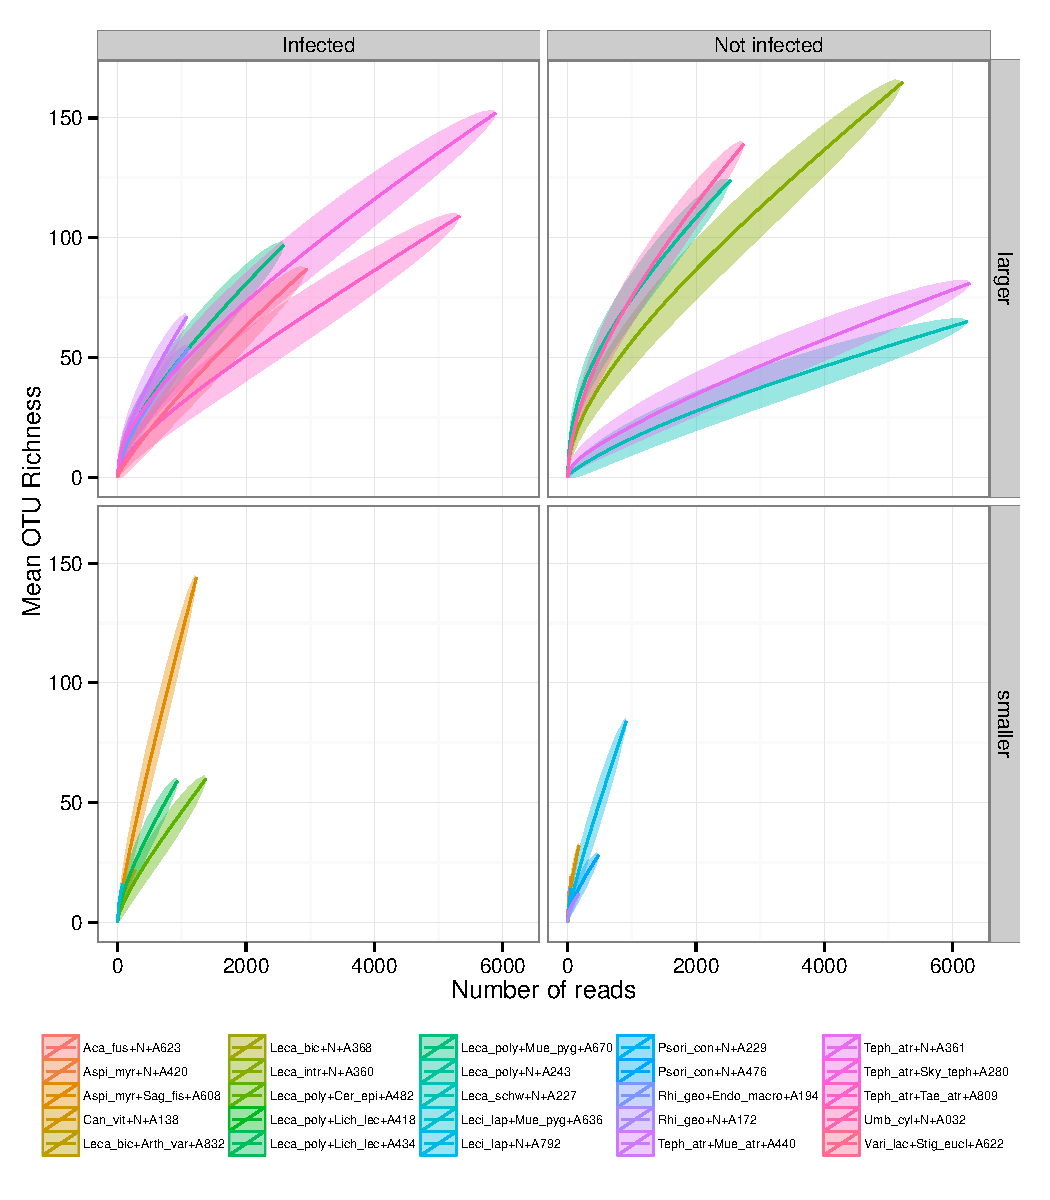
\includegraphics[width=\maxwidth]{figure/rarefact-1} \caption[Rarefaction curves of OTU richness per samples]{Rarefaction curves of OTU richness per samples. All singletons were included.}\label{fig:rarefact}
\end{figure}


\end{knitrout}
%
%
\begin{knitrout}
\definecolor{shadecolor}{rgb}{0.969, 0.969, 0.969}\color{fgcolor}\begin{figure}[H]
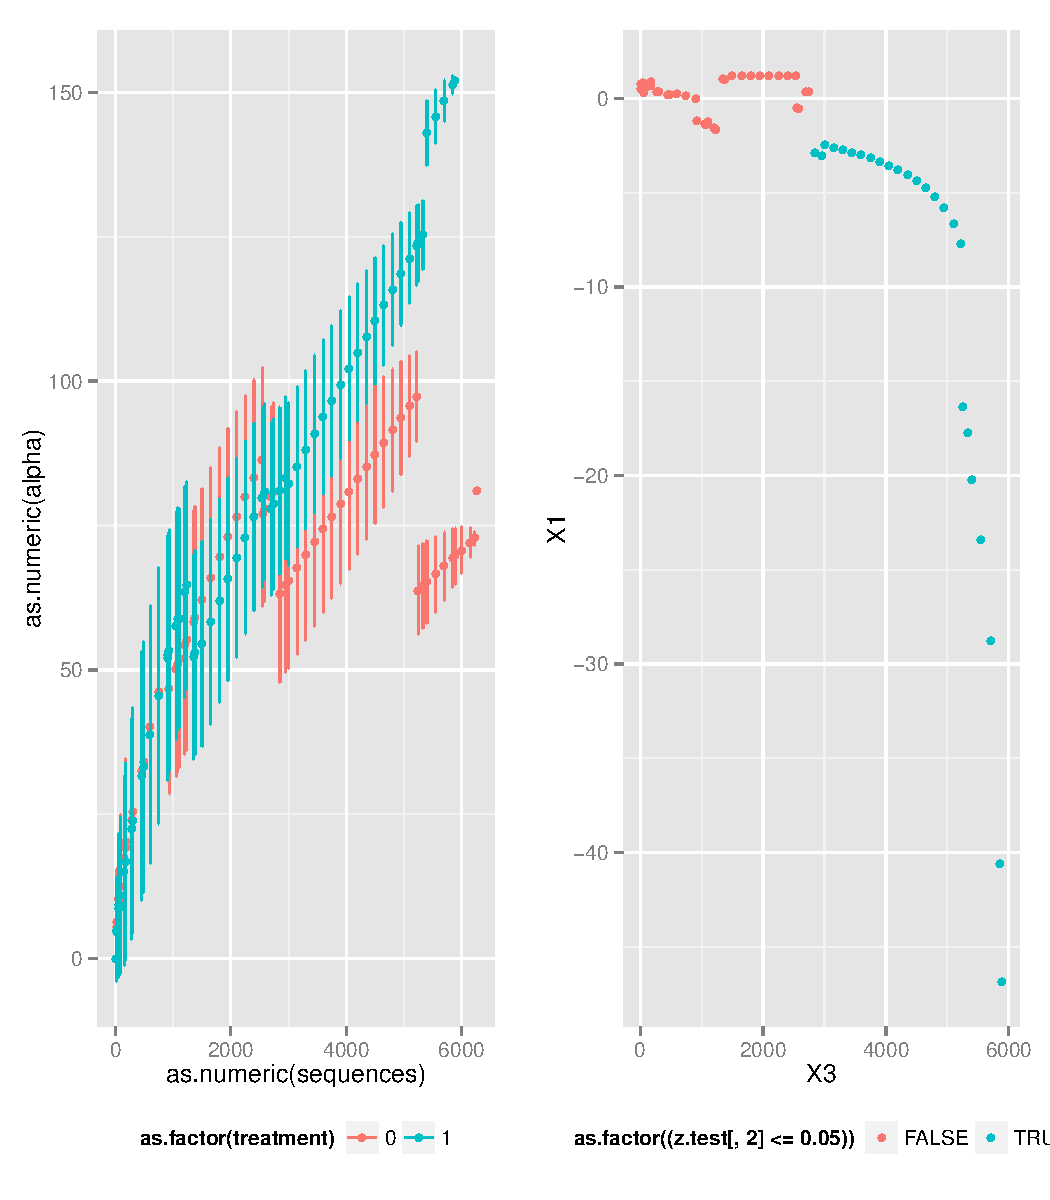
\includegraphics[width=\maxwidth]{figure/rarefact1a-1} \caption[Average rarefied OTU Richness per treatment]{Average rarefied OTU Richness per treatment. All singletons were included.}\label{fig:rarefact1a}
\end{figure}


\end{knitrout}


\begin{knitrout}
\definecolor{shadecolor}{rgb}{0.969, 0.969, 0.969}\color{fgcolor}\begin{figure}[H]
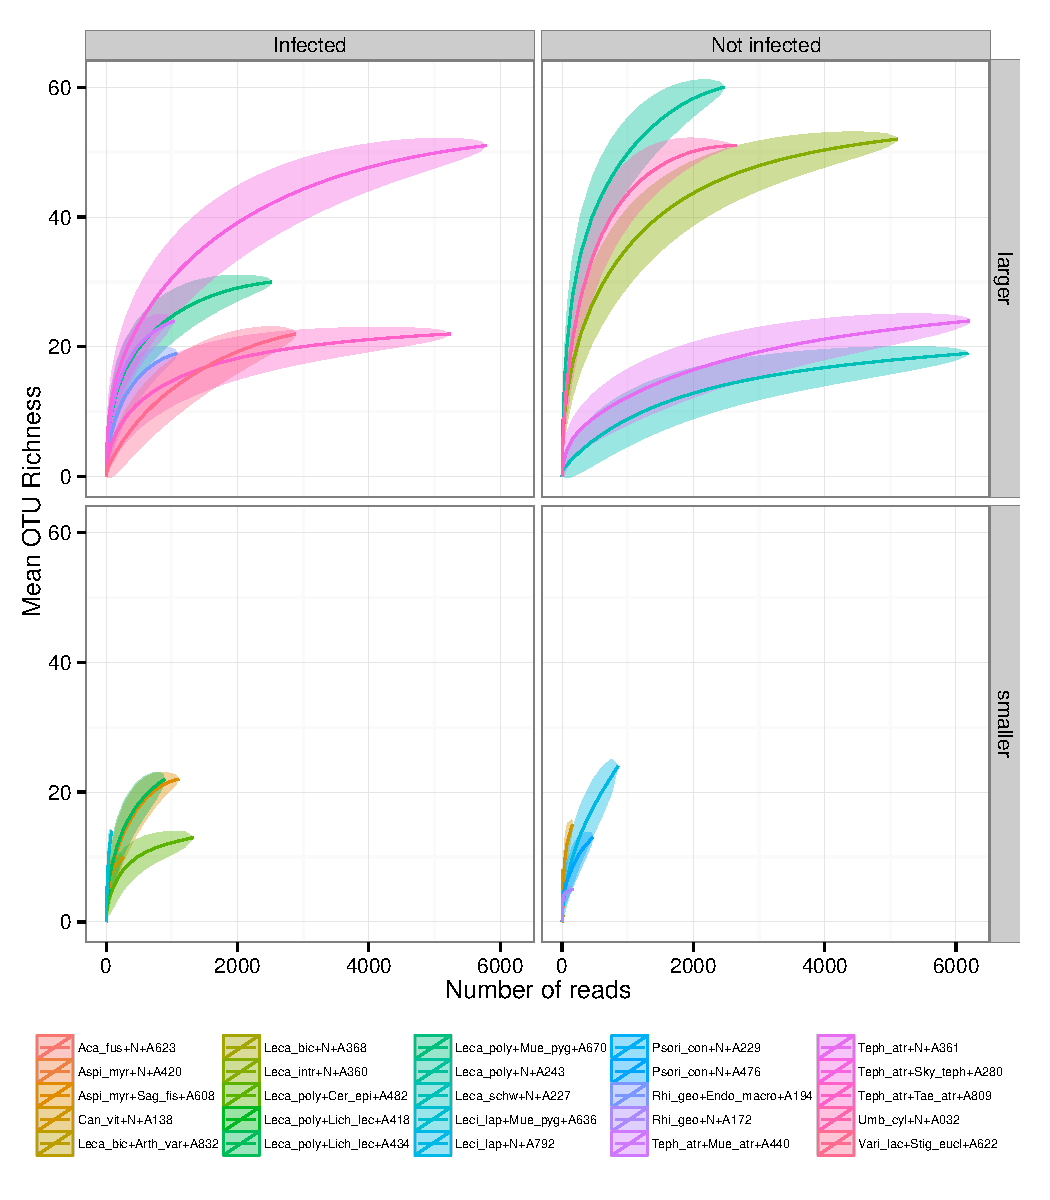
\includegraphics[width=\maxwidth]{figure/rarefact2-1} \caption[Rarefaction curves of OTU richness per samples]{Rarefaction curves of OTU richness per samples. All singletons were excluded.}\label{fig:rarefact2}
\end{figure}


\end{knitrout}
\begin{knitrout}
\definecolor{shadecolor}{rgb}{0.969, 0.969, 0.969}\color{fgcolor}\begin{figure}[H]
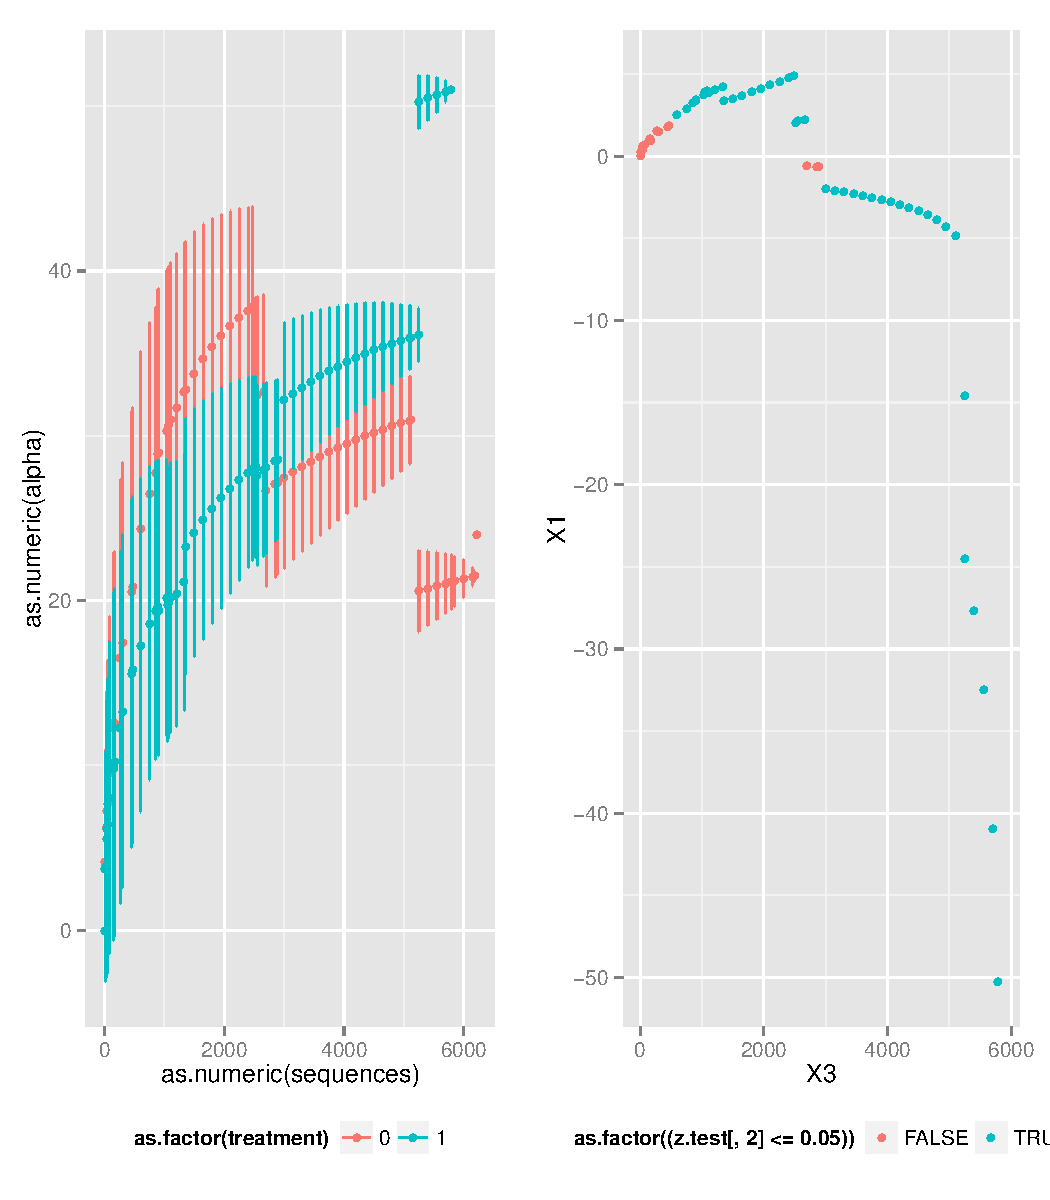
\includegraphics[width=\maxwidth]{figure/rarefact2a-1} \caption[Average rarefied OTU Richness per treatment]{Average rarefied OTU Richness per treatment. All singletons were excluded.}\label{fig:rarefact2a}
\end{figure}


\end{knitrout}

\subsection{Taxonomic Diversity and rarefaction curves}

At Order level

\begin{knitrout}
\definecolor{shadecolor}{rgb}{0.969, 0.969, 0.969}\color{fgcolor}\begin{figure}[H]
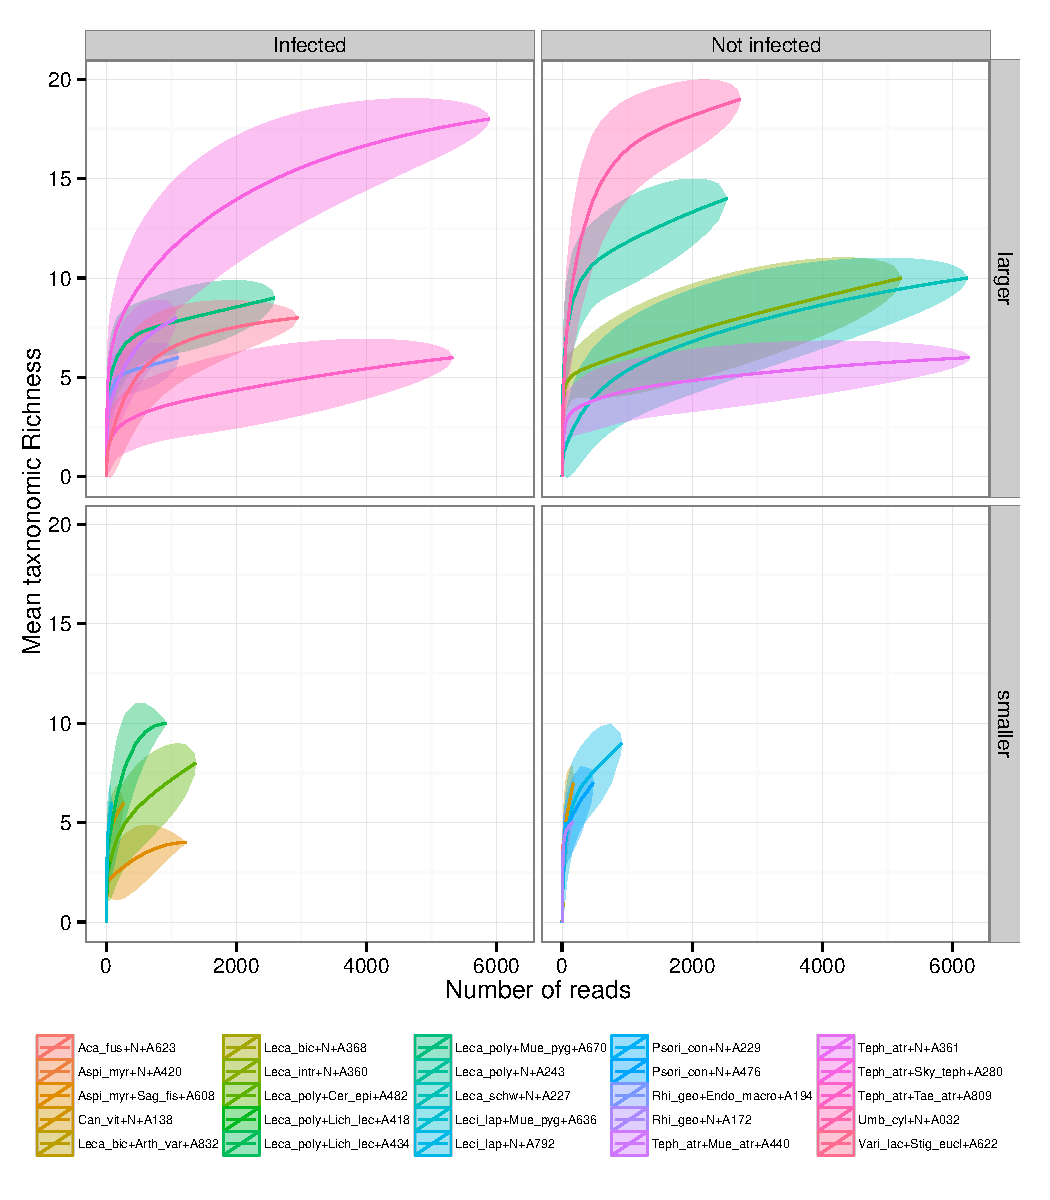
\includegraphics[width=\maxwidth]{figure/rarefact_Orders-1} \caption[Rarefaction curves of Taxonomic richness at Order level per sample]{Rarefaction curves of Taxonomic richness at Order level per sample}\label{fig:rarefact_Orders}
\end{figure}


\end{knitrout}

\begin{knitrout}
\definecolor{shadecolor}{rgb}{0.969, 0.969, 0.969}\color{fgcolor}\begin{figure}[H]
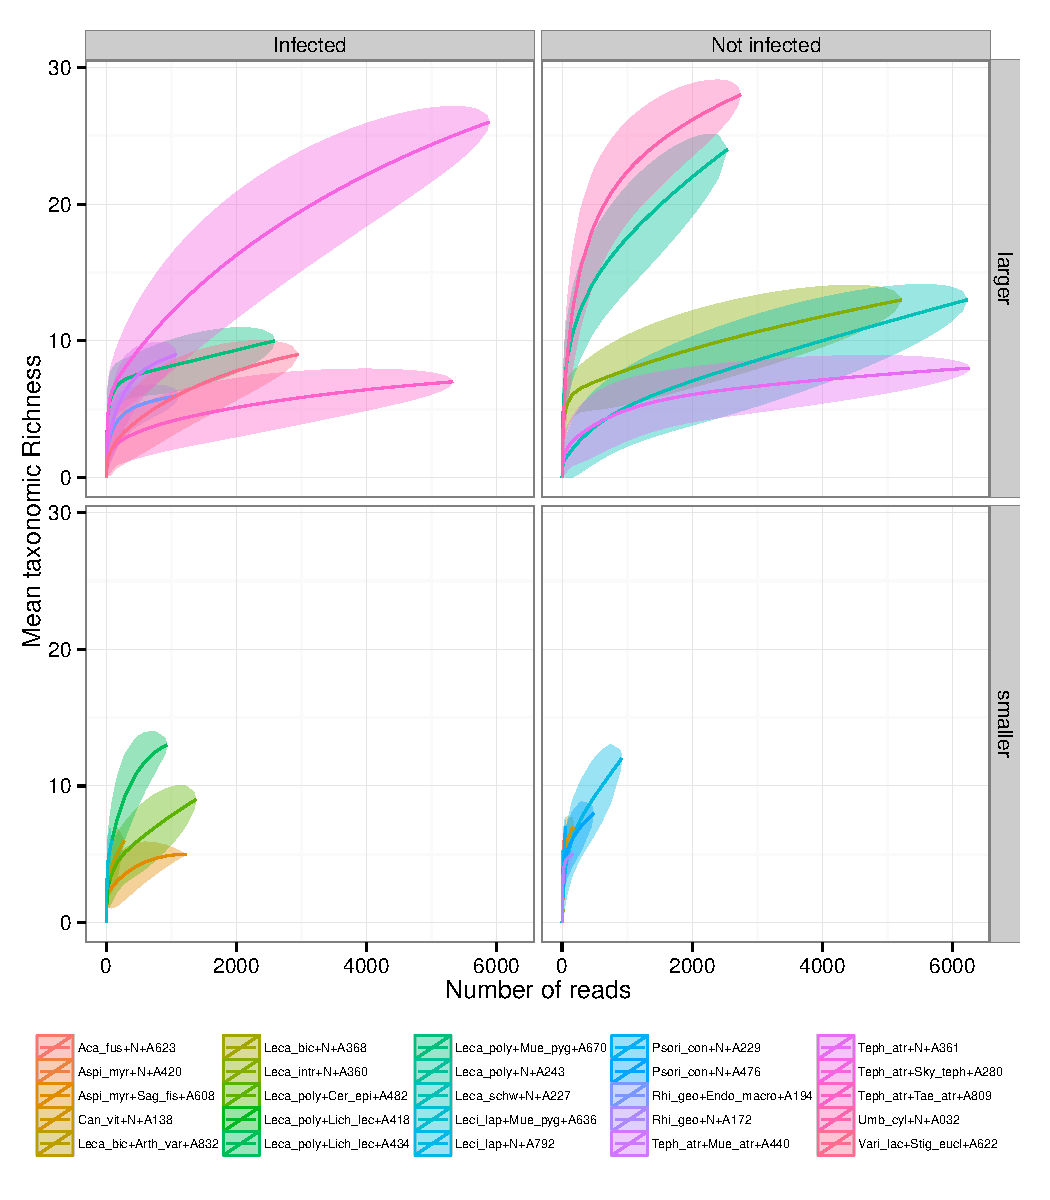
\includegraphics[width=\maxwidth]{figure/rarefact_Families-1} \caption[Rarefaction curves of Taxonomic richness at Family level per sample]{Rarefaction curves of Taxonomic richness at Family level per sample}\label{fig:rarefact_Families}
\end{figure}


\end{knitrout}
\begin{knitrout}
\definecolor{shadecolor}{rgb}{0.969, 0.969, 0.969}\color{fgcolor}\begin{figure}[H]
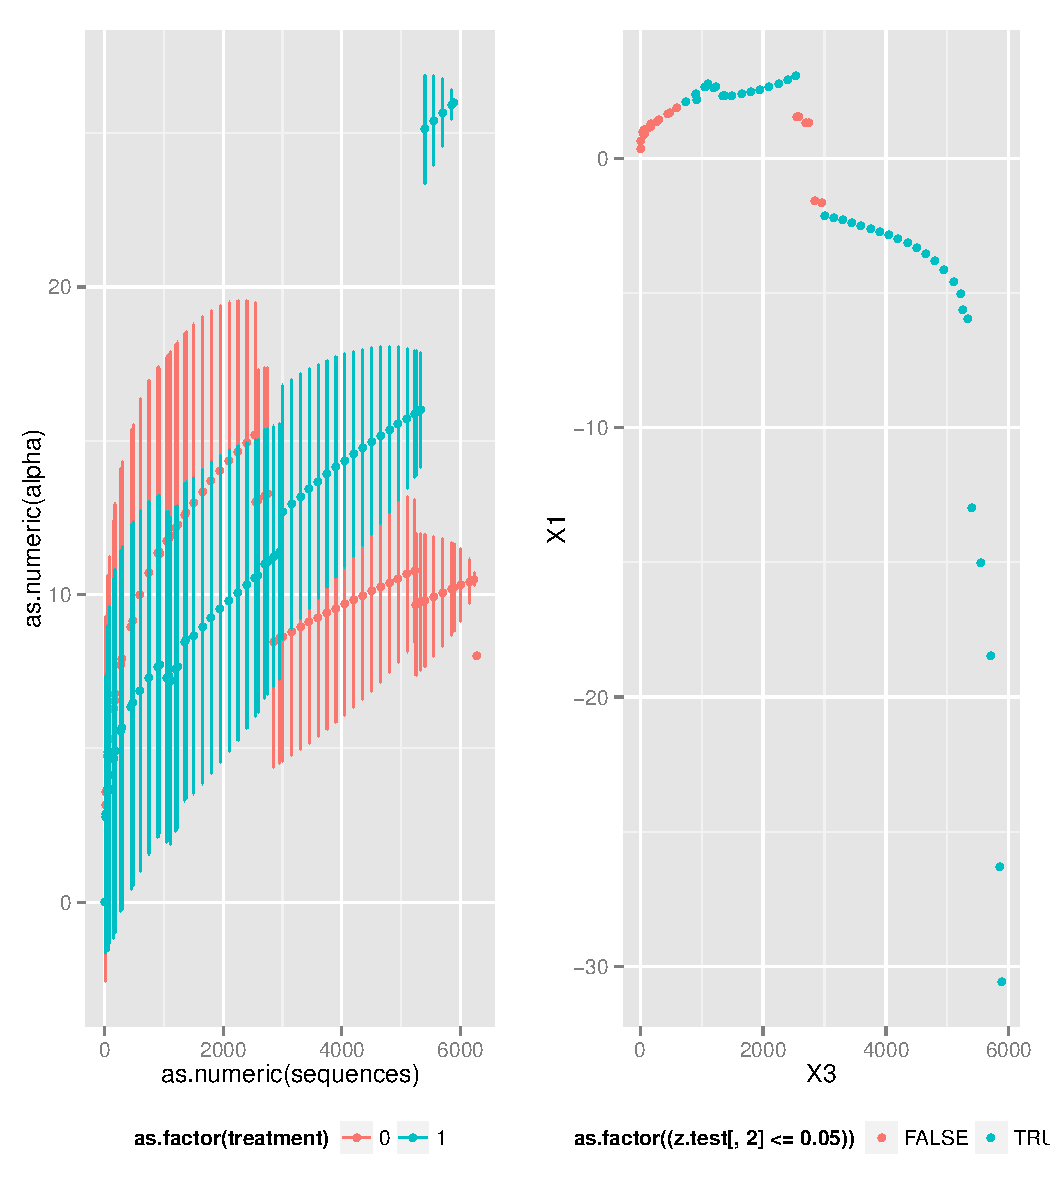
\includegraphics[width=\maxwidth]{figure/rarefact_Orders1a-1} \caption[Average rarefied OTU Richness per treatment]{Average rarefied OTU Richness per treatment. All singletons were included.}\label{fig:rarefact_Orders1a}
\end{figure}


\end{knitrout}
%
%
%
\begin{knitrout}
\definecolor{shadecolor}{rgb}{0.969, 0.969, 0.969}\color{fgcolor}\begin{figure}[H]
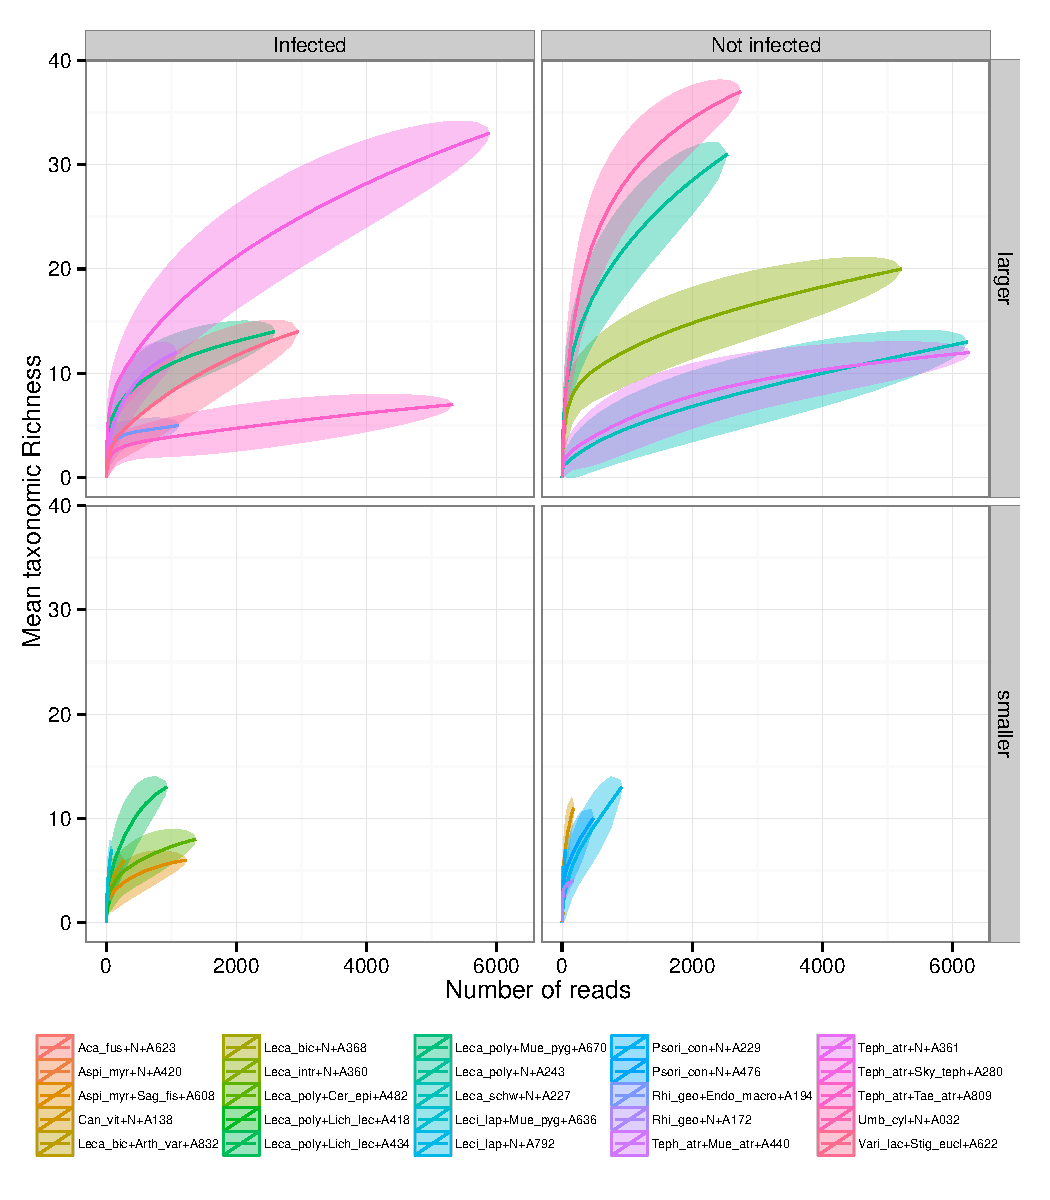
\includegraphics[width=\maxwidth]{figure/rarefact_genera-1} \caption[Rarefaction curves of Taxonomic richness at genus level per sample]{Rarefaction curves of Taxonomic richness at genus level per sample}\label{fig:rarefact_genera}
\end{figure}


\end{knitrout}
%
% PSEUDOSPECIES
%
\begin{knitrout}
\definecolor{shadecolor}{rgb}{0.969, 0.969, 0.969}\color{fgcolor}\begin{figure}[H]
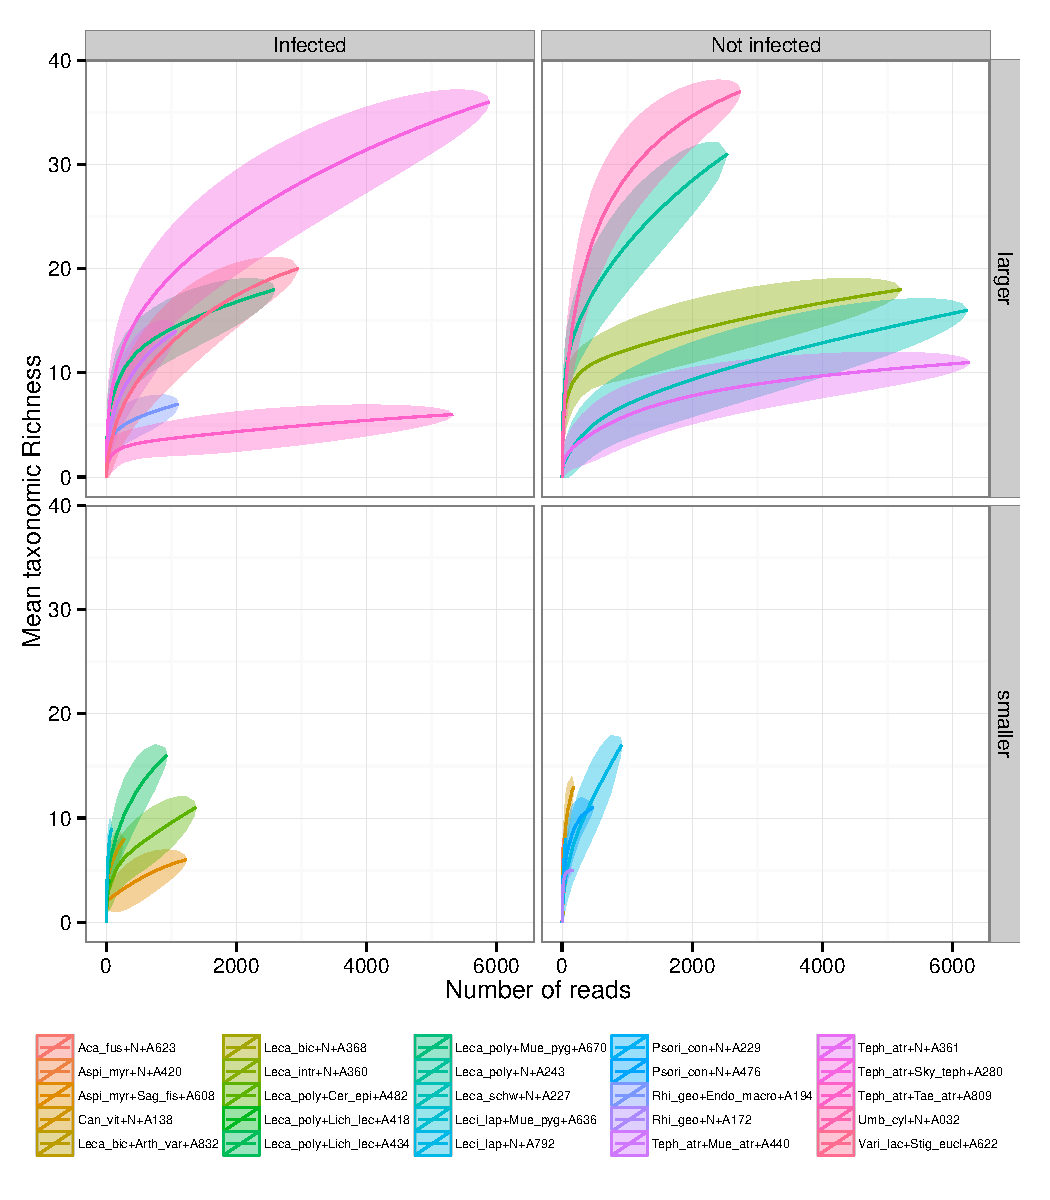
\includegraphics[width=\maxwidth]{figure/rarefact_species-1} \caption[Rarefaction curves of Taxonomic richness at Pseudospecies level per sample]{Rarefaction curves of Taxonomic richness at Pseudospecies level per sample}\label{fig:rarefact_species}
\end{figure}


\end{knitrout}
\section{Clasification of samples based on OTU composition}
\begin{knitrout}
\definecolor{shadecolor}{rgb}{0.969, 0.969, 0.969}\color{fgcolor}\begin{figure}[H]
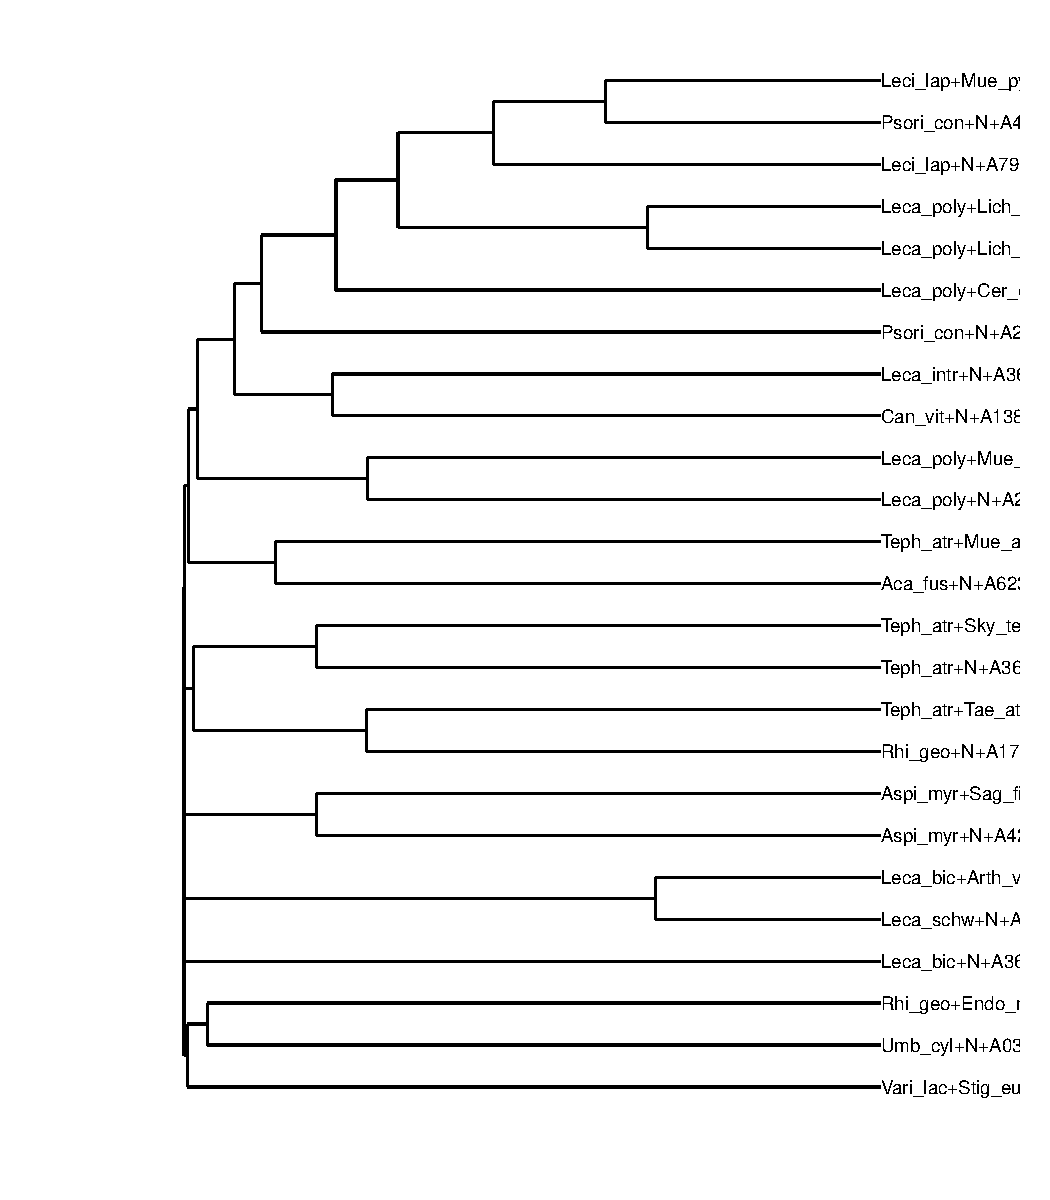
\includegraphics[width=\maxwidth]{figure/foo_tree-1} \caption[Hierarchical clustergram (dendrogram) showing similarity in OTU composition between samples]{Hierarchical clustergram (dendrogram) showing similarity in OTU composition between samples. Hierarchical clustering was carried out on a pairwise Bray-Curtis distance matrix between samples. The long branch lengths of the cladogram reinforce the lack of structure of the dataset. Bray-Curtis distances tend to overestimate the differences due to minoritary species}\label{fig:foo_tree}
\end{figure}


\end{knitrout}

% latex table generated in R 3.0.3 by xtable 1.7-4 package
% Mon Feb 20 14:10:12 2017
\begin{sidewaystable}[b]
\centering
\caption[Exclusive and shared OTUS]{Exclusive and shared OTUS between samples. First column shows the total number OTUs and the number of of heavy OTUs, the second column the number of Exclusive OTUS and the rest the pattern of shared units.} 
\begin{tabular}{rlllllllllllllllllllllllllll}
  \hline
 & \begin{sideways} Total \end{sideways} & \begin{sideways} Exclusive \end{sideways} & \begin{sideways} A623 \end{sideways} & \begin{sideways} A420 \end{sideways} & \begin{sideways} A138 \end{sideways} & \begin{sideways} A368 \end{sideways} & \begin{sideways} A360 \end{sideways} & \begin{sideways} A243 \end{sideways} & \begin{sideways} A227 \end{sideways} & \begin{sideways} A792 \end{sideways} & \begin{sideways} A229 \end{sideways} & \begin{sideways} A476 \end{sideways} & \begin{sideways} A172 \end{sideways} & \begin{sideways} A361 \end{sideways} & \begin{sideways} A032 \end{sideways} & \begin{sideways} A608 \end{sideways} & \begin{sideways} A832 \end{sideways} & \begin{sideways} A482 \end{sideways} & \begin{sideways} A418 \end{sideways} & \begin{sideways} A434 \end{sideways} & \begin{sideways} A670 \end{sideways} & \begin{sideways} A636 \end{sideways} & \begin{sideways} A194 \end{sideways} & \begin{sideways} A440 \end{sideways} & \begin{sideways} A280 \end{sideways} & \begin{sideways} A809 \end{sideways} & \begin{sideways} A622 \end{sideways} \\ 
  \hline
A623 & 13/8 & 8/1 & . & . & 2 & . & 3 & 5 & 1 & 2 & 1 & 1 & 2 & 3 & 1 & 1 & . & 1 & 1 & 2 & 4 & 3 & 3 & 4 & 5 & 2 & 2 \\ 
  A420 & 19/4 & 17/0 & . & . & 1 & . & . & . & 1 & . & . & 1 & . & . & . & 3 & 1 & 1 & . & 1 & 1 & . & . & 1 & . & . & . \\ 
  A138 & 32/15 & 21/2 & 2 & 1 & . & . & 6 & 4 & 4 & 7 & 2 & 5 & 3 & 6 & 3 & 1 & . & 5 & 2 & 2 & 6 & 4 & 3 & 5 & 5 & 3 & 4 \\ 
  A368 & 2/1 & 3/0 & . & . & . & . & . & . & . & . & . & . & . & . & . & . & . & . & . & 1 & . & . & . & . & . & . & . \\ 
  A360 & 165/52 & 137/22 & 3 & . & 6 & . & . & 13 & 6 & 8 & 4 & 6 & 4 & 13 & 6 & 2 & 2 & 4 & 3 & 7 & 7 & 5 & 8 & 7 & 10 & 5 & 7 \\ 
  A243 & 124/60 & 90/24 & 5 & . & 4 & . & 13 & . & 5 & 14 & 3 & 6 & 3 & 6 & 2 & 2 & . & 3 & 2 & 5 & 8 & 13 & 4 & 7 & 14 & 5 & 7 \\ 
  A227 & 65/19 & 53/5 & 1 & 1 & 4 & . & 6 & 5 & . & 2 & 4 & 3 & 1 & 7 & 3 & 1 & 3 & 3 & 1 & 3 & 6 & 2 & 2 & 3 & 6 & 1 & 3 \\ 
  A792 & 84/24 & 64/2 & 2 & . & 7 & . & 8 & 14 & 2 & . & 2 & 7 & 2 & 5 & 2 & 3 & . & 3 & 3 & 6 & 4 & 9 & 2 & 3 & 11 & 4 & 4 \\ 
  A229 & 14/6 & 10/0 & 1 & . & 2 & . & 4 & 3 & 4 & 2 & . & 2 & 1 & 1 & 1 & . & . & 1 & 1 & 1 & 2 & 2 & 2 & 1 & 2 & 1 & 1 \\ 
  A476 & 28/13 & 17/0 & 1 & 1 & 5 & . & 6 & 6 & 3 & 7 & 2 & . & 2 & 5 & 4 & 1 & . & 4 & 2 & 5 & 5 & 3 & 2 & 7 & 8 & 2 & 3 \\ 
  A172 & 12/5 & 10/1 & 2 & . & 3 & . & 4 & 3 & 1 & 2 & 1 & 2 & . & 3 & 1 & 1 & . & 2 & 1 & 2 & 3 & 2 & 2 & 3 & 3 & 2 & 2 \\ 
  A361 & 81/24 & 60/1 & 3 & . & 6 & . & 13 & 6 & 7 & 5 & 1 & 5 & 3 & . & 6 & 2 & 2 & 6 & 2 & 4 & 5 & 3 & 7 & 10 & 14 & 6 & 7 \\ 
  A032 & 139/51 & 124/34 & 1 & . & 3 & . & 6 & 2 & 3 & 2 & 1 & 4 & 1 & 6 & . & . & 1 & 2 & . & 4 & 9 & 1 & 4 & 3 & 10 & . & 3 \\ 
  A608 & 144/22 & 137/13 & 1 & 3 & 1 & . & 2 & 2 & 1 & 3 & . & 1 & 1 & 2 & . & . & 2 & 1 & . & 2 & 3 & 2 & . & 1 & 3 & 1 & 1 \\ 
  A832 & 22/10 & 18/4 & . & 1 & . & . & 2 & . & 3 & . & . & . & . & 2 & 1 & 2 & . & 1 & . & 1 & 1 & . & . & . & . & . & . \\ 
  A482 & 60/13 & 53/4 & 1 & 1 & 5 & . & 4 & 3 & 3 & 3 & 1 & 4 & 2 & 6 & 2 & 1 & 1 & . & 2 & 4 & 3 & 2 & 1 & 4 & 3 & 3 & 1 \\ 
  A418 & 14/5 & 11/0 & 1 & . & 2 & . & 3 & 2 & 1 & 3 & 1 & 2 & 1 & 2 & . & . & . & 2 & . & 2 & 2 & 1 & 1 & 2 & 1 & 2 & . \\ 
  A434 & 59/22 & 44/5 & 2 & 1 & 2 & 1 & 7 & 5 & 3 & 6 & 1 & 5 & 2 & 4 & 4 & 2 & 1 & 4 & 2 & . & 5 & 2 & 2 & 5 & 8 & 3 & 2 \\ 
  A670 & 97/30 & 77/8 & 4 & 1 & 6 & . & 7 & 8 & 6 & 4 & 2 & 5 & 3 & 5 & 9 & 3 & 1 & 3 & 2 & 5 & . & 4 & 5 & 4 & 9 & 2 & 4 \\ 
  A636 & 16/14 & 4/0 & 3 & . & 4 & . & 5 & 13 & 2 & 9 & 2 & 3 & 2 & 3 & 1 & 2 & . & 2 & 1 & 2 & 4 & . & 1 & 2 & 5 & 2 & 2 \\ 
  A194 & 54/19 & 44/7 & 3 & . & 3 & . & 8 & 4 & 2 & 2 & 2 & 2 & 2 & 7 & 4 & . & . & 1 & 1 & 2 & 5 & 1 & . & 6 & 8 & 3 & 7 \\ 
  A440 & 67/24 & 52/7 & 4 & 1 & 5 & . & 7 & 7 & 3 & 3 & 1 & 7 & 3 & 10 & 3 & 1 & . & 4 & 2 & 5 & 4 & 2 & 6 & . & 12 & 4 & 7 \\ 
  A280 & 152/51 & 120/17 & 5 & . & 5 & . & 10 & 14 & 6 & 11 & 2 & 8 & 3 & 14 & 10 & 3 & . & 3 & 1 & 8 & 9 & 5 & 8 & 12 & . & 5 & 10 \\ 
  A809 & 109/22 & 102/13 & 2 & . & 3 & . & 5 & 5 & 1 & 4 & 1 & 2 & 2 & 6 & . & 1 & . & 3 & 2 & 3 & 2 & 2 & 3 & 4 & 5 & . & 3 \\ 
  A622 & 87/22 & 75/8 & 2 & . & 4 & . & 7 & 7 & 3 & 4 & 1 & 3 & 2 & 7 & 3 & 1 & . & 1 & . & 2 & 4 & 2 & 7 & 7 & 10 & 3 & . \\ 
   \hline
\end{tabular}
\end{sidewaystable}


%@
\end{document}
